\documentclass{amsart}
\usepackage{amsmath,amsfonts,amssymb,latexsym}
\usepackage[margin=1in]{geometry}
\usepackage{color}
\usepackage[pagebackref, bookmarks=true, bookmarksopen=true, bookmarksdepth=3,bookmarksopenlevel=2, colorlinks=true, linkcolor=blue, citecolor=blue, filecolor=blue, menucolor=blue, urlcolor=blue]{hyperref}
\input xy
\xyoption{all}
\usepackage{tikz}
\usetikzlibrary{calc}

\usepackage[inline]{showlabels}

\newtheorem{theorem}{Theorem}[section]
\newtheorem{corollary}[theorem]{Corollary}
\newtheorem{definition}[theorem]{Definition}
\newtheorem{lemma}[theorem]{Lemma}
\newtheorem{question}[theorem]{Question}
\newtheorem{proposition}[theorem]{Proposition}
\newtheorem{remark}[theorem]{Remark}
\newtheorem{example}[theorem]{Example}

\numberwithin{equation}{section}

\newcommand{\bfa}{\mathbf{a}}
\newcommand{\bfb}{\mathbf{b}}
\newcommand{\bfc}{\mathbf{c}}
\newcommand{\bfe}{\mathbf{e}}
\newcommand{\bfp}{\mathbf{p}}
\newcommand{\bfq}{\mathbf{q}}
\newcommand{\bfr}{\mathbf{r}}
\newcommand{\bfs}{\mathbf{s}}
\newcommand{\bft}{\mathbf{t}}
\newcommand{\bfu}{\mathbf{u}}
\newcommand{\bfv}{\mathbf{v}}
\newcommand{\bfx}{{\boldsymbol{x}}}
\newcommand{\bfy}{{\boldsymbol{y}}}

\newcommand{\cA}{\mathcal{A}}
\newcommand{\cB}{\mathcal{B}}
\newcommand{\cD}{\mathcal{D}}
\newcommand{\cF}{\mathcal{F}}
\newcommand{\cG}{\mathcal{G}}
%\newcommand{\cH}{\mathcal{H}}
\newcommand{\cL}{\mathcal{L}}
\newcommand{\cO}{\mathcal{O}}
\newcommand{\cP}{\mathcal{P}}
\newcommand{\cT}{\mathcal{T}}
\newcommand{\cU}{\mathcal{U}}
\newcommand{\cX}{\mathcal{X}}

\newcommand{\CC}{\mathbb{C}}
\newcommand{\FF}{\mathbb{F}}
\newcommand{\kk}{\Bbbk}
\newcommand{\PP}{\mathbb{P}}
\newcommand{\QQ}{\mathbb{Q}}
\newcommand{\RR}{\mathbb{R}}
\newcommand{\TT}{\mathbb{T}}
\newcommand{\ZZ}{\mathbb{Z}}

\newcommand{\diag}{\operatorname{diag}}
\newcommand{\Hom}{\operatorname{Hom}}
\newcommand{\Li}{\operatorname{Li}}
\newcommand{\Lie}{\operatorname{Lie}}
\renewcommand{\max}{\operatorname{max}}
\newcommand{\Spec}{\operatorname{Spec}}

\newcommand{\rra}{\rightrightarrows}

\newcommand{\erase[1]}{{}}

\title{Symplectic Groupoids for Cluster Manifolds}
\author{Songhao Li}
\address[Songhao Li]{University of Notre Dame, Department of Mathematics, Notre Dame, IN 46556, USA}
\email{sli19@nd.edu}

\author{Dylan Rupel}
\address[Dylan Rupel]{University of Notre Dame, Department of Mathematics, Notre Dame, IN 46556, USA}
\email{drupel@nd.edu}

\begin{document}
\begin{abstract}
  We construct a source simply-connected symplectic groupoid integrating a log-canonical Poisson structure on a cluster manifold.
\end{abstract}
\maketitle
Outline
\begin{enumerate}
	\item Intro to cluster algebra and compatible Poisson structures 
	\item Intro to Poisson manifolds, symplectic groupoid and Poisson spray
	\item Cluster symplectic groupoid
	\item Totally positive cluster manifolds (definition of manifolds with corners [check D Joyce], associahedron of type A and generalized associahedron)
	\item Examples
\end{enumerate}

%%%%%%%%%%%%%%%%%%%%%%
\section{Introduction}
This is the first of a series of papers whose aim is to implement a modified version of Weinstein's program of geometric quantization for Poisson manifolds \cite{MR1104934} in the case of cluster Poisson structures.
In this first paper, we construct the symplectic groupoids for both the cluster $\cA$-varieties and the cluster $\cX$-varieties. 

The cluster $\cA$-varieties are the geometric realization of cluster algebras defined by Fomin and Zelevinsky \cite{FZ02} as the culmination of their study of total positivity and canonical bases for algebraic groups.
Many varieties arising in Lie theory, e.g.\ Grassmannians and double Bruhat cells, are examples of $\cA$-varieties \cite{berenstein-fomin-zelevinsky,scott,gekhtman-shapiro-vainshtein,williams}.
The cluster $\cA$-varieties are often endowed with a class of compatible Poisson structures in the sense of Gekhtman, Shapiro, and Vainshtein \cite{GSV10}.

The cluster $\cX$-varieties were introduced by Fock and Goncharov \cite{FG09a} in their study of higher Teichmuller space.
The $\cX$-varieties are always endowed with a canonical Poisson structure.
If a $\cA$-variety carries a compatible Poisson structure, then the natural map from this $\cA$-variety to the corresponding $\cX$-variety is Poisson.

In the case of cluster algebras, the quantum $\cA$-varieties \cite{berenstein-zelevinsky} and the quantum $\cX$-varieties \cite{FG09c} are both concrete examples of deformation quantization of Poisson manifolds \cite{MR2062626}.
Geometric quantization for symplectic manifolds takes one step further by constructing an action on a Hilbert space, but this requires that the cohomology class of the symplectic 2-form be integral (see e.g.\ \cite{MR1806388}).
The notion of symplectic groupoids was introduced by Weinstein \cite{MR866024}, Karas\"{e}v \cite{MR1008479} and Zakrzewski \cite{MR1081010, MR1081011}.
Weinstein's motivation was to find a geometric quantization schema for Poisson manifolds \cite{MR1104934}, which has only been successfully implemented for a handful of examples \cite{MR2417440, MR2925830}.
The concrete nature of cluster coordinates makes that setting an ideal testing ground for groupoid quantization.
Indeed, a modified version was implicitly implemented by Fock and Goncharov \cite{FG09c} in the case of $\cX$-varieties.

In this paper, we take the first step towards the groupoid quantization for both $\cA$-varieties and $\cX$-varieties, by constructing their symplectic groupoids. The paper is organized as follows.

In Section~\ref{sec: local}, we construct three groupoids $\cG$, $\cB$ and $\cD$ for a log canonical Poisson $\pi$ on a vector space $L$. The groupoid $\cG \rra L$ is the source-simply-connected symplectic groupoid. This is essentially the construction of local symplectic groupoids by Poisson sprays \cite{MR2900786, CMS17}. For a log-canonical Poisson structure, there is a nice choice of the Poisson spray such that the construction yields the global source-simply-connected symplectic groupoid $\cG$. Being the source-simply-connected symplectic groupoid, the source and the target maps of $\cG \rra L$ are transcendental.

The groupoid $\cB \rra L$ is a source-connected symplectic groupoid. The advantage of $\cB \rra L$ is that the source and the target maps of $\cG \rra L$ are rational. The tradeoff is the expression symplectic form is more complicated.

The groupoid $\cD \rra L$ is a source-connected Poisson groupoid. The restriction of $\cD \rra L$ over an octant $L_+$ of $L$, which we denote by $\cD_+ \rra L_+$ is symplectic, is called the symplectic double in \cite{FG09c}, albeit with slightly different notations to accommodate the case of the non-square exchange matrices.

The symplectic groupoid $\cB \rra L$ can be realized as the blowup of $\cD \rra L$ in the sense of \cite{MR3214314}, whereas both $\cB \rra L$ and $\cD \rra L$ receives maps from the source-simply-connected symplectic groupoid $\cG$.

In Section~\ref{sec:cluster}, we give the explicit formulae for the cluster groupoid mutation $\mu: \cG \to \cG'$, $\mu: \cB \to \cB'$ and $\mu: \cD \to \cD'$. The first step is to decompose a generalized cluster mutation $\mu: L \to L'$ into two maps $\varphi^1$ and $\tau$. The first map $\varphi^1$ is the time-$1$-flow of a Hamiltonian vector field defined using the Euler dilogarithm function; the second map $\tau$ is a natural transformation of log-canonical coordinates \cite{FG09a, MR3691969}. We then lift $\varphi^1$ and $\tau$ to groupoid maps, and the composition the lifted groupoid maps is the cluster groupoid mutation.

\bigskip


We use the following notations.
\begin{itemize}
	\item We write $\RR_+ = (0, \infty)$, $\bar\RR_+ = [0, \infty)$ and $\CC_\times = \CC \setminus \{0\}$.
	\item For the cluster charts, we use the following notations:
	$$
		L = \RR^m \text{ or } \CC^m, \quad L^+ = \RR_+^m \text{ or } \CC_\times^m, \quad \bar L_+ = \bar\RR_+^m.
	$$
	\item We denote vectors by boldface, e.g. $\bfx = (x_1, \ldots, x_m)$.
	\item Hadamard product: for two vector $\bfx$ and $\bfy$, $\bfx \circ \bfy = (x_1y_1, \ldots, x_my_m)$.
	\item For a vector $\bfx$ and a real number $t$, $\bfx^t = (x_1^t, \ldots, x_m^t)$.
	\item For a vector $\bfx$, we denote the diagonal matrix for which the diagonal entries is $\bfx$ by $I_\bfx$, i.e. 
	\[
		I_\bfx = \begin{bmatrix} x_1 & 0 & \cdots & 0 \\ 0 & x_2 & \cdots & 0 \\ \vdots & \vdots & \ddots & \vdots \\ 0 & 0 & \cdots & x_m \end{bmatrix}
	\]
	\item For a vector bundle $A$ over $M$, we denote the space of sections by $\cA = \Gamma(M, A)$. In particular, we denote the space of vector fields by $\cT_M = \Gamma(M, TM)$, but to follow the conventional notation, we denote the space of differential $1$-forms by $\Omega^1(M) = \Gamma(M, T^*M)$.
	%\item for two vector $\bfx$ and $\bfa$, $\bfx^\bfa = \prod_{i=1}^m x_i^{a_i}$;
	%\item for a matrix $B = (B_{ij})$, $B_{[k]}$ denotes the kth column vector of $B$.
\end{itemize}


%%%%%%%%%%%%%%%%%%%%%%%%%%%%%%%%%%%%%%%%%%%%%%%%%%%%%%%%%%%%%%%%%%
\section{Symplectic groupoids of log-canonical Poisson structures}
\label{sec: local}

%In this section, we will use the idea of Poisson spray \cite{MR2900786} to construct the source-simply-connected sympletic groupoid of a log-canonical Poisson structure.
%There is another construction of a source-connected symplectic groupoid, called the symplectic double \cite{FG09c}.
%We give an explicit formula for the groupoid morphism from the source-simply-connected symplectic groupoid to the symplectic double.
%We recall the natural Poisson map between two compatible log-canonical Poisson structures, which serve as the seeds for cluster $\cA$-varieties and $\cX$-varieties.

We begin with the equivalent notions of Poisson brackets and Poisson bi-vectors.
\begin{definition}
  Let $M$ be either a smooth manifold or a complex manifold.
  A \emph{Poisson structure} on $M$ is one of the two following equivalent structures:
  \begin{enumerate}
    \item a \emph{Poisson bracket}
      $$\{\cdot, \cdot\}: \cO_M \times \cO_M \to \cO_M$$
      which is a Lie bracket satisfying the Leibniz rule
      $$\{fg, h\} = f\{g,h\} + g\{f,h\};$$
    \item a \emph{Poisson bi-vector} $\pi \in \cT^2_M$ such that $[\pi, \pi] = 0$, where $[\cdot, \cdot]$ is the Schouten-Nijenhuis bracket.
  \end{enumerate}
We say $f \in \cO_M$ is a Casimir if $\{f, g\} = 0$ for every $g\in \cO_M$.
\end{definition}

The two notions are related by the formula: $\{f, g\} = \pi (df \otimes dg)$ for $f, g\in \cO_\cX$.
The pair $(M, \pi)$, or equivalently $(M, \{\cdot,\cdot\})$, is called a \emph{Poisson manifold}. A Poisson map from $(M_1, \pi_1)$ to $(M_2, \pi_2)$ is a map $\varphi: M_1\to M_2$ such that $\varphi_*\pi_1 = \pi_2$ or equivalently $\{\varphi^*f, \varphi^*g\} = \varphi^*(\{f, g\})$ for $f, g \in \cO_{M_2}$.

A bi-vector $\pi \in \cT^2_M$ is called \emph{non-degenerate} if the bundle map
\[\pi^\flat: \Omega^1(M) \to \cT_M, \qquad \alpha \mapsto \iota_\alpha \pi\]
is invertible. The inverse of the bundle map defines a non-degenerate 2-form $\omega \in \Omega^2(M)$. That is, the bundle map
\[\omega^\sharp: \cT_M \to \Omega^1(M), \qquad v \mapsto \iota_v \omega\]
is the inverse of $\pi^\flat$. The condition $[\pi,\pi]$ is equivalent to $d\omega = 0$, so a non-degenerate Poisson bi-vector is the same as a symplectic 2-form. Hence for a symplectic 2-form $\omega$, we denote the corresponding Poisson bi-vector as $\omega^{-1}$.

\begin{definition}
For a Poisson manifold $(M, \pi)$, a symplectic realization is a symplectic manifold $(S, \omega)$ together with a surjecive Poisson map $\rho: (S, \omega) \to (M, \pi)$.
\end{definition}

We continue with the notion of Lie groupoids.

\begin{definition}
  A \emph{groupoid} $\cG\rightrightarrows M$ consists of two sets $\cG$ and $M$ with the following maps:
  \begin{enumerate}
    \item a surjective \emph{source map} $\alpha: \cG \to M$ and a surjective \emph{target map} $\beta: \cG \to M$;
    \item an injective identity map $\mathtt{1}: M \to \cG, \enskip x \mapsto \mathtt{1}_x$;
    \item an associative multiplication map $m: \cG {_\beta \times_\alpha} \cG \to \cG, \enskip (g, h) \mapsto gh$;
    \item and an involutive inversion map $\iota: \cG \to \cG, \enskip g \mapsto g^{-1}$;
  \end{enumerate}
  which satisfy the following properties:
  \begin{enumerate}
    \item $\alpha(\mathtt{1}_x) = \beta(\mathtt{1}_x) = x$;
    \item $\alpha(gh) = \alpha(g), \enskip \beta(gh) = \beta(h)$;
    \item $\alpha(g^{-1}) = \beta(g), \enskip \beta(g^{-1}) = \alpha(g)$;
    \item $(\mathtt{1}_x)^{-1} = \mathtt{1}_x$.
  \end{enumerate}
  A \emph{Lie groupoid} $\cG \rightrightarrows M$ has the following additional properties:
  \begin{enumerate}
    \item $\cG$ and $M$ are either smooth manifolds or complex manifolds;
    \item the source $\alpha: \cG \to M$ and the target $\beta: \cG \to M$ are surjective submersions;
    \item the multiplication map $m: \cG {_\beta \times_\alpha} \cG \to \cG$ is smooth;
    \item the inversion map $i: \cG \to \cG$ is smooth.
  \end{enumerate}
  A Lie groupoid $\cG \rightrightarrows M$ is \emph{source-connected} if the source fiber $\alpha^{-1}(x)$ is connected for every $x \in M$; it is \emph{source-simply-connected} if the source fiber $\alpha^{-1}(x)$ is connected and simply-connected for every $x \in M$.
\end{definition}

We recall the notion of a Lie algebroid, which is the infitesimal object of a Lie groupoid.
\begin{definition}
	For a smooth (or holomorphic) manifold $M$, a Lie algebroid over $M$ is a triple $(A, [\cdot, \cdot], \rho)$ where
	\begin{enumerate}
		\item $A$ is a vector bundle over a $M$,
		\item $[\cdot, \cdot]$ is a Lie bracket on the space of section $\cA$ of $A$, and
		\item $\rho: A \to TM$ is a bundle morphism preserving the Lie bracket
	\end{enumerate}
	that satisfies the Leibniz rule: for $X, Y \in \cA$ and $f \in \cO_M$,
	\[
		[X, fY] = \rho(X) f \cdot Y + f[X, Y].
	\]
\end{definition}

There is a Lie functor from the Lie groupoids to the Lie algebroids. For a Lie groupoid $\cG \rra M$, we define its Lie algebroid $A = \Lie \cG$ as follows. As a vector bundle, $A = \ker \left(\alpha_*: T\cG|_{\mathtt{1}_M} \to TM \right)$. The Lie bracket is the bracket of left-invariant vector fields, and the anchor map is $\beta_*: T\cG \to TM$ restricted to $A$. In this case, we say the Lie groupoid $\cG$ integrates the Lie algebroid $A$.

Given a Lie groupoid $\cG \rra M$, its $k$-nerve 
\[
	\cG^{(k)} = \{(g_1, g_2, \ldots, g_k) \in \cG^k ~|~ \beta(g_i) = \alpha(g_{i+1})\}
\]
is the set of $k$ composable elements. In particular, $\cG^{(2)} = \cG {_\beta \times_\alpha} \cG$, $\cG^{(1)} = \cG$ and $\cG^{(0)} = M$. The nerve of a Lie groupoid is naturally a simplicial manifold that carries a coboundary operator $\partial: \Omega^\bullet(\cG^{(k-1)}) \to \Omega^\bullet(\cG^{(k)})$. The first two operators are given as below:
\begin{align} \label{eq:gpdcob}
	& \partial: \Omega^\bullet(M) \to \Omega^\bullet(\cG), \qquad \mu \mapsto \alpha^*(\mu) - \beta^*(\mu) \\
	& \partial: \Omega^\bullet(\cG) \to \Omega^\bullet(\cG^{(2)}), \qquad \mu \mapsto \mathrm{pr}_1^*(\mu) - m^*(\mu) + \mathrm{pr}_2^*(\mu)
\end{align}
where $\mathrm{pr}_1: \cG^{(2)} \to \cG$ and $\mathrm{pr}_2: \cG^{(2)} \to \cG$ are the first and second projections. A differential form $\mu \in \Omega^\bullet(G)$ is called \emph{multiplicative} if $\partial \mu = 0$. Our main interest will be with Lie groupoids equipped with a multiplicative symplectic structure.
\begin{definition}
  A \emph{symplectic groupoid} is a Lie groupoid $\cG \rra M$ with a multiplicative symplectic structure $\omega \in \Omega^2(\cG)$.
  That is, $\mathrm{pr}_1^*(\omega)+\mathrm{pr}_2^*(\omega) = m^*(\omega)$. or equivalently the graph of the multiplication map $\Gamma_m = \{(g, h, gh) \in \cG \times \cG \times \cG\}$ is Lagrangian with repsect to the symplectic structure $\omega \oplus \omega \oplus -\omega$.
\end{definition}

We note that symplectic groupoids is a special case of Poisson groupoids.
\begin{definition}
  A \emph{Poisson groupoid} is a Lie groupoid $\cG \rra M$ with a multiplicative Poisson structure $\omega \in \cT^2_\cG$. That is, the graph of the multiplication map $\Gamma_m$ is coisotropic with repsect to the Poisson structure $\pi \oplus \pi \oplus -\pi$.
\end{definition}

A symplectic groupoid map from $(\cG_1, \omega_1) \rra M_1$ to $(\cG_2, \omega_2) \rra M_2$ is a Lie groupoid map $\varphi: \cG_1 \to \cG_2$ which is also a symplectomorphism. The source fibers of a symplectic groupoid are symplectic orthogonal to the target fibers.

For a symplectic groupoid $(\cG, \omega) \rra M$, there is a natural Poisson structure $\pi$ on $M$ such that $\alpha: (\cG, \omega) \to (M, \pi)$ and $\beta: (\cG, \omega) \to (M, -\pi)$ are symplectic realizations.
Poisson manifolds that arise this way are called \emph{integrable}. The Lie algeboid of a symplectic groupoid $\cG \rra M$ is the cotangent Lie algebroid $T^*M$ \cite{MR866024} with the anchor map
$$
	\pi^\flat: T^*_M \to T_M, \qquad \alpha \mapsto \iota_\alpha \pi,
$$
and the Koszul bracket: for $\alpha, \beta \in \Omega^1(M)$,
$$
	[\alpha, \beta] = \cL_{\pi(\alpha)} \beta - \cL_{\pi(\alpha)} \beta - d\pi(\alpha \otimes \beta).
$$


As a Poisson groupoid, $(\cG, \omega) \rra (M, \pi)$ integrates the Lie bialgebroid $(T^*M, TM)$, where $TM$ carries the standard Lie algebroid structure \cite{MR1262213}.
The integrability of Poisson manifolds, and more generally the integrability of Lie algebroids, is characterized in \cite{MR1973056, MR2128714}.
We list some important examples of symplectic groupoids: the Kostant-Kirillov-Souriau Poisson structures \cite{MR996653}, the Drinfeld double of Poisson Lie groups \cite{MR1054741}, the double Bruhat cells \cite{LuM16}, the blow-up groupoid of log symplectic manifolds \cite{MR3214314}, and the symplectic double of the cluster $\cX$-varieties \cite{FG09c}. %For the two extreme cases where the Poisson structure is either trivial or non-degenerate, we describe the symplectic groupoid below.

%\begin{example}
%	\begin{enumerate}
%	\item Let $M$ be a smooth (or holomorphic) manifold with the trivial Poisson structure, i.e. every function $f\in \cO_M$ is a Casimir. The symplectic groupoid over $M$ is $T^*M$ with the standard symplectic structure, where $\alpha$ and $\beta$ are the bundle projections and the multiplication is the fiberwise addition.
%	\item Let $(M, \omega)$ be a connected symplectic manifold. The pair groupoid $(M \times M, \omega \oplus -\omega)$ is a source-connected symplectic groupoid over $(M, \omega)$ where $\alpha(x,y) = x$, $\beta(x,y) = y$ and $m((x,y), (y,z))=(x,z)$. The fundamental groupoid $\Pi M$ consisting of homotopy paths is the source-simply-connected symplectic groupoid where $\alpha([\gamma]) = \gamma(0)$, $\beta([\gamma]) = \gamma(1)$, the multiplication is the concatenation of paths and with the symplectic structure $\alpha^*\omega - \beta^*\omega$.
%	\end{enumerate}
%\end{example}


Let $(\cG_1, \omega_1) \rra (M_1, \pi_1)$ and $(\cG_2, \omega_2) \rra (M_2, \pi_2)$ be symplectic groupoids.
In general, a Poisson map $\varphi: (M_1, \pi_1) \to (M_2, \pi_2)$ does not integrate to a symplectic groupoid map $\tilde{\varphi}: (\cG_1, \omega_1) \rra (\cG_2, \omega_2)$.
In fact, $\varphi$ being Poisson means that its graph $\Gamma_\varphi \in M_1 \times M_2$ is coisotropic with respect to $\pi \oplus -\pi$ \cite{MR959095} and coisotropic submanifolds integrates to Lagrangian subgroupoids \cite{MR2104442}, so a Poisson map $\varphi: (M_1, \pi_1) \to (M_2, \pi_2)$ integrates to a Lagrangian subgroupoid of $(\cG_1\times\cG_2, \omega_1\oplus-\omega_2)$.
However as a recurring theme throughout \S\ref{sec:cluster}, the cluster mutations always lift to groupoid mutations.

We focus on the symplectic groupoids of log-canonical Poisson structures.

\begin{definition}
  Let $L$ be either $\RR^m$ or $\CC^m$ and write $\bfx = (x_1, \ldots, x_m)$ for a system of coordinates on $L$.
  A Poisson structure on $L$ is \emph{log-canonical} if
  $$
    \{x_i, x_j\} = \Omega_{ij} x_ix_j, \quad 1 \leq i,j \leq m \qquad \text{or equavalently} \quad
    \pi = \sum_{j < i} \Omega_{ij} x_ix_j\frac{\partial}{\partial x_i} \wedge \frac{\partial}{\partial x_j},
  $$
  for some skew-symmetric $m\times m$ matrix $\Omega = (\Omega_{ij})$.
\end{definition}

For both the cluster $\cA$-varieties \cite{GSV10} and $\cX$-varieties \cite{FG09c}, the compatible Poisson structures are log-canonical in cluster charts.
Using the results in \cite{MR2900786, CMS17}, we construct the source-simply-connected symplectic groupoid of a log-canonical Poisson structure by chosing an appropriate Poisson spray. 
\begin{definition} 
  \cite{MR2900786}
  For a Poisson manifold $(M, \pi)$, a \emph{Poisson spray} is a vector field $X \in \cT_{T^*M}$ such that
  \begin{enumerate}
    \item for $(x,p) \in T^*M$ we have
      \[\tau_* X|_{(x,p)} = \pi^\flat(p),\]
      where $\tau: T^*M \to M$ is the bundle projection;
    \item $X$ is homogeneous of degree 1, i.e.
      \[(m_\lambda)_*(X) = \lambda X,\]
      where $m_\lambda: T^*M \to T^*M, \enskip (x,p) \mapsto (x,\lambda p)$ is the fiberwise scaling map.
  \end{enumerate}
\end{definition}

\begin{theorem} 
  \cite{MR2900786, CMS17} 
  \label{thm:poissp}
  For a smooth Poisson manifold $(M, \pi)$ with a Poisson spray $X \in \cT_{T^*M}$, a neighbourhood $U$ of the zero section of $T^*M$ is a local symplectic groupoid over $(M, \pi)$ with the following structures:
  \begin{enumerate}
    \item the source map $\alpha: U \to M$ is the bundle projection;
    \item the target map is
      \[\beta: U \to M, \qquad \beta = \tau \circ \varphi_X^1,\]
      where $\varphi_X^1: T^*M \to T^*M$ is the time-$1$-flow of $X$;
    \item the identity map $\mathtt{1}: M \to U$ is the zero section;
    \item the inverse map is
      \[\iota: U \to U, \qquad \iota = -\varphi_X^1;\]
    \item the multiplication $m: U {_\beta \times_\alpha} U \to U$ is defined as the solution of an ODE (see \cite{CMS17} for details);
    \item the symplectic form on $U$ is
      \[\omega = \int_{0}^{1} (\varphi_X^s)^*\omega_0 ds,\]
      where $\omega_0$ is the standard symplectic structure on $T^*M$.
  \end{enumerate}
\end{theorem}

\begin{remark}
For the standard symplectic structure $\omega_0$ in Theorem~\ref{thm:poissp}, we use the sign convention that $\omega_0 = - d \theta_0$ where $\theta_0$ is the tautological 1-form on $T^*M$. This choice ensures that the source map $\alpha$ is Poisson. In coordinates, we have $\omega_0 = \sum_i d x_i \wedge d p_i$.
\end{remark}

\begin{remark}
By a local symplectic groupoid $(\cG, \omega) \rra (M, \pi)$, we mean that the multiplication $m: \cG {_\beta \times_\alpha} \cG \to \cG$ may not be defined on all of its domain. In general, the local symplectic groupoid structure cannot be extended to the total space $T^*M$. Indeed: the Poisson spray $X$ may not be complete; the flow of the Poisson spray $X$ may contain loops; or the 2-form $\omega$, though non-degenerate near the zero section of $T^*M$, may be degenerate in general.
\end{remark}

In the next results, we introduce a Poisson spray whose local symplectic groupoid provides an integration of a log-canonical Poisson structure.
\begin{lemma}
  For the log-canonical Poisson structure $\{x_i, x_j\} = \Omega_{ij} x_i x_j$ on $L = \RR^m$, the vector field $X \in \cT_{T^*L}$ given by
  \begin{equation} 
    \label{eq: PoisSp}
    X = \sum_{1 \leq i,j \leq m}\Omega_{ij}x_i p_i x_j\frac{\partial}{\partial x_j} - \sum_{1 \leq i,j \leq m}\Omega_{ij}x_ip_i p_j\frac{\partial}{\partial p_j}
  \end{equation}
  is a Poisson spray.
  Its flow is given by
  \[\varphi_X^t: T^*L \to T^*L, \qquad (\bfp, \bfx) \mapsto (\bfa^{-t} \circ \bfp, \bfa^t \circ \bfx),\]
  where $a_j = e^{\sum_i \Omega_{ij} x_ip_i}$.
  This flow exists for all time $t \in \RR$ and contains no loops.
\end{lemma}

\begin{proof}
  For the co-vector $\alpha = p_1 dx_1 + \ldots + p_m dx_m$ and the point $(\mathbf{x}, \mathbf{p})$, we have
  \[\tau_* X|_{(\mathbf{x},\mathbf{p})} = \sum_{i, j}\Omega_{ij} x_i p_i x_j \frac{\partial}{\partial x_j} = \iota_\alpha \pi.\]
  To find the flow of $X$, we note that $x_i p_i$ is a constant under the flow of $X$:
  \[\frac{d}{dt}(x_j p_j) = \dot{x}_j p_j - x_j \dot{p}_j = \sum_{1 \leq i,j \leq m}\Omega_{ij}x_i p_i x_j p_j - \sum_{1 \leq i,j \leq m}\Omega_{ij}x_ip_i p_j x_j = 0.\]
  Therefore $\sum_{i}\Omega_{ij}x_i p_i$ is constant, and
  \begin{align*}
    x_j(t) & = e^{t \sum_i \Omega_{ij} x_ip_i} x_j(0) = a_j^t x_j(0), \\
    p_j(t) & = e^{-t \sum_i \Omega_{ij} x_ip_i} p_j(0) = a_j^{-t} p_j(0).
  \end{align*}
\end{proof}

This Poisson spray $X$ induces the symplectic groupoid structure below.
\begin{theorem} 
  \label{thm:PoiSpLogC}
  For the log-canonical Poisson structure $\{x_i, x_j\} = \Omega_{ij} x_i x_j$ on $L$ (which is either $\RR^m$ or $\CC^m$), there is a source-simply-connected symplectic groupoid $(\cG, \omega_\cG) \rra (L, \pi)$ with the following structures:
  \begin{enumerate}
    \item $\cG \cong T^*L$ has the coordinates $(\bfp, \bfx) = (p_1, \ldots, p_m, x_1, \ldots, x_m)$;
    \item the source map is the bundle projection $\alpha: T^*L \to L, \quad (\bfp, \bfx) \mapsto \bfx$;
    \item the target map is $\beta: T^*L \to L, \quad (\bfp, \bfx) \mapsto \bfa \circ \bfx$, where $a_j = e^{\sum_i \Omega_{ij} x_ip_i}$;
    \item the identity map $\mathtt{1}: L \to T^*L, \quad \bfx \mapsto (0, \bfx)$;
    \item the inverse map is $\iota: T^*L \to T^*L, \quad (\bfp, \bfx) \mapsto -\bfa^{-1}\circ \bfx$;
    \item the multiplication map is $m: T^*L {_\alpha \times_\beta} T^*L \to T^*L, \quad \big((\bfp, \bfx), (\bfp', \bfa \circ \bfx)\big) \mapsto (\bfa \circ \bfp' + \bfp, \bfx )$;
    \item the multiplicative symplectic form $\omega$ is
      \begin{equation}
	\omega_\cG = \sum_{i} dx_i \wedge dp_i + \sum_{i, j} \Omega_{ij}p_ix_j dx_i \wedge dp_j + \sum_{j < i} \Omega_{ij}p_ip_j dx_i \wedge dx_j + \sum_{j < i} \Omega_{ij}x_ix_j dp_i \wedge dp_j, 
      \end{equation}
      or equivalently
      \begin{equation}
      \label{eq:2-formGA}
      	\pi_\cG = \omega_\cG^{-1} = \sum_{i} \frac{\partial}{\partial p_i} \wedge \frac{\partial}{\partial x_i} - \sum_{i, j} \Omega_{ij}p_i x_j \frac{\partial}{\partial p_i} \wedge \frac{\partial}{\partial x_j} +\sum_{j < i} \Omega_{ij}p_ip_j \frac{\partial}{\partial p_i} \wedge \frac{\partial}{\partial p_j} +\sum_{j < i} \Omega_{ij}x_ix_j \frac{\partial}{\partial x_i} \wedge \frac{\partial}{\partial x_j}.
      \end{equation}
  \end{enumerate}
\end{theorem}
\begin{proof}
  When the underlying field is $\RR$, it is straightforward to check that the Poisson spray \eqref{eq: PoisSp} induces the given groupoid structures. To find the sympletic structure $\omega_\cG$, we have
\begin{align*}
		\left(\varphi_X^s\right)^*\omega_0 & = \sum_{j} d \left(e^{ s \sum_{i} \Omega_{ij} x_ip_i}x_j \right) \wedge d \left(e^{- s \sum_{i} \Omega_{ij} x_ip_i}p_j \right) \\
		& = \sum_{j} \left(s x_j \sum_{i} \Omega_{ij} x_i dp_i + s x_j \sum_{i} \Omega_{ij} p_i dx_i + d x_j \right) \wedge \left(- s p_j \sum_{i} \Omega_{ij} x_i dp_i - s p_j \sum_{i} \Omega_{ij} p_i dx_i + d p_j \right) \\
		& = \sum_{j} dx_j \wedge dp_j + 2s \left( \sum_{i, j} \Omega_{ij}p_i x_j d x_i \wedge d p_j  + \sum_{j < i} \Omega_{ij}p_ip_j d x_i \wedge d x_j + \sum_{j < i} \Omega_{ij}x_ix_j d p_i \wedge d p_j \right),
\end{align*}
so it follows that
\begin{align*}
		\omega_\cG & = \int_{0}^{1} (\varphi_X^s)^*\omega_0 ds \\
		& = \sum_{i} dx_i \wedge dp_i
	  + \left(
	    \sum_{i, j} \Omega_{ij}p_ix_j dx_i \wedge dp_j 
	    + \sum_{j < i} \Omega_{ij}p_ip_j dx_i \wedge dx_j
	    + \sum_{j < i} \Omega_{ij}x_ix_j dp_i \wedge dp_j
	  \right).
	\end{align*}
Note that $\omega_\cG$ is non-degenerate since
  \[(\omega_\cG)^m = m! \bigwedge\limits_{1\leq i\leq m} dx_i \wedge dp_i\]
  is a volume form.

  In the case when the underlying field is $\CC$, the symplectic groupoid structures can be verified directly.
\end{proof}

Motiviated by \cite{FG09c}, we make the following definition of the symplectic double, which is a source-connected Poisson groupoid of the log-canonical Poisson structure on $L$.
\begin{theorem} \label{thm:SymDBLoc}
  \cite{FG09c}
  For the log-canonical Poisson structure $\{x_i, x_j\} = \Omega_{ij} x_i x_j$ on $L$ (which is either $\RR^m$ or $\CC^m$), the \emph{symplectic double} $(\cD, \omega_\cD) \rra (L, \pi)$ is a source-connected Poisson groupoid with the following structures:
  \begin{enumerate}
    \item $\cD \cong L_+ \times L$ (where $L_+$ is either $\RR_+^m$ or $\CC_\times^m$) has the coordinates $(\bfs, \bfx) = (s_1, \ldots, s_m, x_1, \ldots, x_m)$;
    \item the source map is
      \[\alpha: L_+ \times L \to L, \qquad (\bfs, \bfx) \mapsto \bfx;\]
    \item the target map is
      \[\beta: L_+ \times L \to L, \qquad (\bfs, \bfx) \mapsto \left(x_1 \prod_{i=1}^m s_i^{\Omega_{i1}}, \ldots, x_m \prod_{i=1}^m s_i^{\Omega_{im}}\right);\]
	\item the identity map $\mathtt{1}: L \to L_+ \times L, \quad \bfx \mapsto (1, \ldots, 1, \bfx)$;
    \item the inverse map is
      \[\iota: L_+ \times L \to L_+ \times L, \qquad (\bfs, \bfx) \mapsto \left(\frac{1}{s_1}, \ldots, \frac{1}{s_m}, x_1 \prod_{i=1}^m s_i^{\Omega_{i1}}, \ldots, x_m \prod_{i=1}^m s_i^{\Omega_{im}}\right);\]
    \item the multiplication map is
      \[\begin{aligned}
	  m: & \left(L_+ \times L\right) {_\beta \times_\alpha} \left(L_+ \times L\right) \to L_+ \times L, \\
	     & \left((\bfs, \bfx), \left(\bfs', x_1 \prod_{i=1}^m s_i^{\Omega_{i1}}, \ldots, x_m \prod_{i=1}^m s_i^{\Omega_{im}}\right)\right) \mapsto (\bfs' \circ \bfs, \bfx );
        \end{aligned}\]
    \item the multiplicative Poisson structure is
    \begin{equation}
    \label{eq:2-formGX}
		\pi_\cD =\sum_{i} s_ix_i\frac{\partial}{\partial s_i} \wedge \frac{\partial}{\partial x_i}+\sum_{j < i} \Omega_{ij}x_ix_j \frac{\partial}{\partial x_i} \wedge \frac{\partial}{\partial x_j}
    \end{equation}
    or equivalently the singular multiplicative 2-form $\omega_\cD$ is
      \begin{equation} 
	\omega_\cD = \pi_\cD^{-1} = \sum_{i} \frac{dx_i}{x_i} \wedge \frac{ds_i}{s_i} + \sum_{j < i} \Omega_{ij} \frac{ds_i}{s_i} \wedge \frac{ds_j}{s_j}.
      \end{equation}
  \end{enumerate}
\end{theorem}

It may be strange that the Poisson groupoid $\cD \rra L$ is called the symplectic double. The symplectic double in \cite{FG09c} is defined to be the restriction $\cD_+ =\{(\bfs, \bfx) ~|~ \bfx \in L_+ \} \cong L_+ \times L_+$ which is genuinely a symplectic groupoid over $L_+$. The Poisson groupoid $\cD \rra L$ may be thought as the natural extension of the symplectic groupoid $\cD_+ \rra L_+$.

\begin{remark}
	We relate the target map in Theorem~\ref{thm:SymDBLoc} to the symplectic realization in \cite{MR3691969}.
	
	With the notations in Theorem~\ref{thm:SymDBLoc} and the change of variables $e^{\chi_i} = x_i$ and $e^{\xi_i} = s_i$, the symplectic double $(\cD, \omega_\cD)$ becomes the symplectic vector space $(\cU, \omega_\cU)$ where $\cU$, with coordinates $(\xi_1, \ldots, \xi_m, \chi_1, \ldots, \chi_m)$, is either $\RR^{2m}$ or $\CC^{2m}$ and
	\[
		\omega_\cU = \sum_{i} d\chi_i \wedge d\xi_i + \sum_{j < i} \Omega_{ij} d\xi_i \wedge d\xi_j.
	\]
Although $(\cU, \omega_\cU)$ is not a symplectic groupoid of $(L, \pi)$ (e.g. the identity map cannot be defined), the maps $\alpha$ and $\beta$ are well-defined in these coordinates:
	\begin{align*}
		& \alpha: \cU \to L, \qquad (\xi_1, \ldots, \xi_m, \chi_1, \ldots, \chi_m) \mapsto \left(e^{\chi_1}, \ldots, e^{\chi_m}\right), \\
		& \beta: \cU \to L, \qquad (\xi_1, \ldots, \xi_m, \chi_1, \ldots, \chi_m) \mapsto \left(e^{\chi_1+\sum_i\Omega_{i1}\xi_i}, \ldots, e^{\chi_m+\sum_i\Omega_{im}\xi_i}\right),
	\end{align*}
The $\alpha$-fibers are symplectic orthogonal to the $\beta$-fibers; both $\alpha: (\cU, \omega_\cU) \to (L, \pi)$ and $\beta: (\cU, - \omega_\cU) \to (L, \pi)$ are Poisson maps.

For the standard symplectic structure $\omega_0 = \sum_{i} d\chi_i \wedge d\xi_i$ on $\cU$, since
	\[
		\omega - \omega_0 = \left(\sum_{i} d\chi_i \wedge d\xi_i + \sum_{j < i} \Omega_{ij} d\xi_i \wedge d\xi_j \right) - \sum_{i} d\chi_i \wedge d\xi_i  =\sum_{j < i} \Omega_{ij} d\xi_i \wedge d\xi_j
	\]
is supported on the $\alpha$-fiber, it follows that $\beta_*(-\omega_0^{-1}) = \beta_*(-\omega_\cU^{-1}) = \pi$. The symplectic realization $\beta: (\cU, -\omega_0) \to (L, \pi)$ plays an important role in \cite{MR3691969}.
\end{remark}

Next, we describe the Lie algebroid of $\cD \rra L$. We write $A_\cD \cong L\times L$ as a vector bundle over $L$ where the bundle projection is $(\bfs, \bfx) \mapsto \bfx$. For a $m\times m$ skew-symmetric matrix $\Omega$, we define the Lie algebroid $A_\cD \cong L\times L$ over $L$ with the anchor map
\[
	A_\cD \cong L\times L \to TL, \qquad (\bfs, \bfx) \mapsto \sum_{i,j}x_i\Omega_{ij}s_j\frac{\partial}{\partial x_j}.
\]


For a $m\times m$ skew-symmetric matrix $\Omega$, $\bfx \in L$ and $\bfs \in L_+$, we define the matrix
\[
	I_\bfx \Omega I_\bfs^{-1} = \begin{bmatrix} \frac{x_1\Omega_{11}}{s_1} & \frac{x_1\Omega_{12}}{s_2} & \cdots & \frac{x_1\Omega_{1m}}{s_m} \\ \frac{x_2\Omega_{21}}{s_1} & \frac{x_2\Omega_{22}}{s_2} & \cdots & \frac{x_2\Omega_{2m}}{s_m} \\ \vdots & \vdots & \ddots & \vdots \\ \frac{x_m\Omega_{m1}}{s_1} & \frac{x_m\Omega_{m2}}{s_2} & \cdots & \frac{x_m\Omega_{mm}}{s_m} \end{bmatrix}
\]


We take a degression... elementary modification... blowup...

For an integrable Lie algebroid, every source-connected integration receives a surjective groupoid map from the source-simply-connected groupoid.
With our chosen conventions, we have a simple expression for the groupoid map $\cG \to \cD$.
\begin{proposition}
  As symplectic groupoids over the log Poisson structure on $\RR_+^m$ or $(\CC^\times)^m$, the map
  \[
  	\kappa: \cG \to \cD, \qquad (\bfp, \bfx) \mapsto (e^{x_1p_1}, \ldots, e^{x_mp_m}, \bfx)
  \]
  is a symplectic groupoid morphism.
\end{proposition}

\begin{proof}
We show that $\kappa$ is compatible with the target maps, and leave the compatibility with other structure maps to the readers.
	\begin{align*}
		(\beta_\cD \circ \kappa) (\bfp, \bfx) & = \beta_\cD (e^{x_1p_1}, \ldots, e^{x_mp_m}, \bfx) \\
		& = \left(x_1 \prod_{i=1}^m e^{\Omega_{i1}x_ip_i}, \ldots, x_m \prod_{i=1}^m e^{\Omega_{im}x_ip_i}\right) \\
		& = \left(x_1 e^{\sum_i \Omega_{i1}x_ip_i}, \ldots, x_m  e^{\sum_i \Omega_{im}x_ip_i}\right) \\
		& = \beta_\cG (\bfp, \bfx).
	\end{align*}
To show that $\kappa$ preserves the symplectic structures, we have
	\begin{align*}
		\kappa^*\omega_\cD & = \sum_{i} \frac{dx_i}{x_i} \wedge \frac{d(e^{x_ip_i})}{e^{x_ip_i}} + \sum_{j < i} \Omega_{ij} \frac{d(e^{x_ip_i})}{e^{x_ip_i}} \wedge \frac{d(e^{x_jp_j})}{e^{x_jp_j}} \\
		& = \sum_{i} \frac{dx_i}{x_i} \wedge (x_i dp_i + p_i dx_i) + \sum_{j < i} \Omega_{ij} (x_i dp_i + p_i dx_i) \wedge (x_j dp_j + p_j dx_j) \\
		& = \sum_{i} dx_i \wedge dp_i
	  	+ \left(
	    	\sum_{i, j} \Omega_{ij}p_ix_j dx_i \wedge dp_j 
	    	+ \sum_{j < i} \Omega_{ij}p_ip_j dx_i \wedge dx_j
	    	+ \sum_{j < i} \Omega_{ij}x_ix_j dp_i \wedge dp_j
	  	\right) \\
		& = \omega_\cG.
	\end{align*}
\end{proof}

The symplectic groupoids $\cG \rra L$ and $\cD \rra L$ are summarized in the following commutative diagram.
\begin{equation} 
    \label{eq:LGpdCD}
    \xymatrix{
      (\cG, \omega_{\cG})  \ar[r]^{\kappa} \ar@/^-0.5pc/[d]|-{\alpha} \ar@/^0.5pc/[d]|-{\beta} & (\cD, \omega_{\cD}) \ar@/^-0.5pc/[d]|-{\alpha} \ar@/^0.5pc/[d]|-{\beta} \\
       (L, \pi) \ar[u]|-{\mathtt{1}} \ar[r]^{=} & (L, \pi) \ar[u]|-{\mathtt{1}}
    }
\end{equation}


%%%%%%%%%%%%%%%%%%%%%%%%%%%%%%%%%%%%%%%%%%%%%%
\section{Hamiltonian Perspective on Mutations}
\label{sec:cluster}

In this section, we introduce mutations of cluster seeds from the Hamiltonian viewpoint.
This perspective was first given in \cite{FG09c} and is the foundation for the main results of \cite{MR3691969}.
We demonstrate how the Hamiltonian perspective provides a canonical choice of mutations for groupoid charts which glue to give a symplectic groupoid integrating various log-canonical Poisson structures on cluster varieties.

Let $\tilde B=(B_{ij})$ be an $m\times n$ integer matrix with $m\ge n$.  
Write $B$ for the upper $n\times n$ submatrix of $\tilde B$ and assume $B$ is skew-symmetrizable, i.e.\ there exists a diagonal integer matrix $D=\diag(d_1,\ldots,d_n)$ with each $d_i>0$ so that $DB$ is skew-symmetric. 
Such an $m\times n$ matrix $\tilde B$ with skew-symmetrizable principal submatrix $B$ is called an \emph{exchange matrix}.
We fix a skew-symmetrizing matrix $D$ and refer to a skew-symmetric $m\times m$ matrix $\Omega=(\Omega_{ij})$ as \emph{$D$-compatible} with $\tilde B$ if $\tilde B^T\Omega=[D\ \boldsymbol{0}]$, where $\boldsymbol{0}$ denotes an $n\times(m-n)$ matrix with all zero entries.
In this case, we call $(\tilde B,\Omega)$ a \emph{$D$-compatible pair}.

\subsection{Mutation of Cluster Charts}
We begin by recalling the Hamiltonian perspective of mutations for cluster charts.
Let $L_\cX=\RR_+^n$ and $L_\cA=\RR_+^m$.
Write $\bfy=(y_1,\ldots,y_n)$ for a set of coordinates on $L_\cX$ and $\bfx=(x_1,\ldots,x_m)$ for a set of coordinates on $L_\cA$.
Given a $D$-compatible pair of matrices $(\tilde B,\Omega)$, denote by $\{\cdot,\cdot\}_\cX$ and $\{\cdot,\cdot\}_\cA$ the log-canonical Poisson brackets on $L_\cX$ and $L_\cA$ given by
\begin{equation}
  \label{eq:brackets}
  \{y_k,y_\ell\}_\cX=d_kB_{k\ell}y_ky_\ell\qquad\text{and}\qquad\{x_i,x_j\}_\cA=\Omega_{ij}x_ix_j.
\end{equation}
An easy calculation shows that there is a Poisson map
\[\rho:L_\cA\to L_\cX,\qquad \rho^*(y_k)=\hat y_k:=\prod_{i=1}^m x_i^{B_{ik}},\]
i.e.\ $\{\hat y_k,\hat y_\ell\}_\cA=d_kB_{k\ell}\hat y_k\hat y_\ell$ for $1\le k,\ell\le n$.
Motivated by the terminology of Fock and Goncharov \cite{FG09a}, we will refer to the pair of Poisson manifolds $L_\cX$ and $L_\cA$ together with the Poisson map $\rho$ as a \emph{Poisson ensemble} associated to the $D$-compatible pair $(\tilde B,\Omega)$.

The \emph{Euler dilogarithm} is the function of a single real variable defined by
\[\Li_2(y)=-\int_0^y \frac{\log(1-u)}{u}du,\qquad y<1.\]
It will become apparent from the results below that, from the Poisson perspective, the Euler dilogarithm lies at the heart of cluster algebra theory.
However, we will work in a slightly more general setting.

Fix a collection of positive integers $\bfr=(r_1,\ldots,r_n)\in\ZZ_{>0}^n$ and write $L_\bfr=\prod_{\ell=1}^n \RR_+^{r_\ell-1}$ with coordinates $a_{\ell,j}$ for $1\le\ell\le n$, $1\le j\le r_\ell-1$.
We identify the $\ell$-th component of a point in $L_\bfr$ with the degree $r_\ell$ monic polynomial $F_\ell(z)\in\RR_+[z]$ with $F_\ell(0)=1$ given by
\[F_\ell(z)=1+a_{\ell,1}z+\cdots+a_{\ell,r_\ell-1}z^{r_\ell-1}+z^{r_\ell}.\]
Set 
\[L_{\cX,\bfr}:=L_\cX\times L_\bfr\qquad\text{ and }\qquad L_{\cA,\bfr}:=L_\cA\times L_\bfr.\]
Here we extend the Poisson structures on $L_\cX$ and $L_\cA$ to $L_{\cX,\bfr}$ and $L_{\cA,\bfr}$ so that the functions $a_{\ell,j}$ on $L_\bfr$ are Casimirs. 
Then the map $\rho:L_\cA\to L_\cX$ extends to a Poisson map $L_{\cA,\bfr}\to L_{\cX,\bfr}$ which we still denote by $\rho$.

Given a choice of sign $\varepsilon\in\{\pm1\}$, define Hamiltonian functions $h^{k,\varepsilon}_{\cX,\bfr}\in\cO_{L_{\cX,\bfr}}$ and $h^{k,\varepsilon}_{\cA,\bfr}\in\cO_{L_{\cA,\bfr}}$ for $1\le k\le n$ by
\begin{equation}
  \label{eq:hamiltonians}
  h_{\cX,\bfr}^{k,\varepsilon}:=-\frac{\varepsilon}{d_k}\int_0^{y_k^\varepsilon} \frac{\log\big(F_k(u)\big)}{u}du\qquad\text{and}\qquad h_{\cA,\bfr}^{k,\varepsilon}:=-\frac{\varepsilon}{d_k}\int_0^{\hat y_k^\varepsilon} \frac{\log\big(F_k(u)\big)}{u}du.
\end{equation}
Observe that when $r_k=1$, i.e.\ $F_k(z)=1+z$, we have $h_{\cX,\bfr}^{k,\varepsilon}:=\frac{\varepsilon}{d_k}\Li_2(-y_k^\varepsilon)$ and $h_{\cA,\bfr}^{k,\varepsilon}:=\frac{\varepsilon}{d_k}\Li_2(-\hat y_k^\varepsilon)$.

Clearly, there is an equality $\rho^*(h_{\cX,\bfr}^{k,\varepsilon})=h_{\cA,\bfr}^{k,\varepsilon}$.
Write $X_{\cX,\bfr}^{k,\varepsilon}\in\cT_{L_{\cX,\bfr}}$ and $X_{\cA,\bfr}^{k,\varepsilon}\in\cT_{L_{\cA,\bfr}}$ for the Hamiltonian vector fields associated to $h_{\cX,\bfr}^{k,\varepsilon}$ and $h_{\cA,\bfr}^{k,\varepsilon}$ respectively, i.e.\ the vector fields naturally associated to the derivations $\{h_{\cX,\bfr}^{k,\varepsilon},\cdot\}_\cX$ and $\{h_{\cA,\bfr}^{k,\varepsilon},\cdot\}_\cA$.
\begin{lemma}
  \label{le:hamiltonian dynamics}
  For $1\le k\le n$ and $\varepsilon\in\{\pm1\}$, the vector fields $X_{\cX,\bfr}^{k,\varepsilon}$ and $X_{\cA,\bfr}^{k,\varepsilon}$ determine the following dynamics on $L_{\cX,\bfr}$ and $L_{\cA,\bfr}$:
  \begin{align}
    \label{eq:X dynamics}
    \dot y_\ell&:=\{h_{\cX,\bfr}^{k,\varepsilon},y_\ell\}_\cX=-B_{k\ell}\log\big(F_k(y_k^\varepsilon)\big)y_\ell\quad\text{for}\quad 1\le\ell\le n;\\
    \label{eq:A dynamics}
    \dot x_j&:=\{h_{\cA,\bfr}^{k,\varepsilon},x_j\}_\cA=-\delta_{jk}\log\big(F_k(\hat y_k^\varepsilon)\big)x_k\quad\text{for}\quad 1\le j\le m.
  \end{align}
  Moreover, the points of $L_\bfr$ are fixed by the Hamiltonian flows.
\end{lemma}
\begin{proof}
  Equation~\eqref{eq:X dynamics} was essentially proven in \cite{MR3691969}.
  Since equation~\eqref{eq:A dynamics} seems to technically be new, we will indicate the key steps in the computation here:
  \[\{h_{\cA,\bfr}^{k,\varepsilon},x_j\}_\cA=-\frac{\log\big(F_k(\hat y_k^\varepsilon)\big)}{d_k\hat y_k}\{\hat y_k,x_j\}=-\delta_{jk}\log\big(F_k(\hat y_k^\varepsilon)\big)x_j.\]
\end{proof}

It immediately follows that $y_k$ is a conserved quantity under the flow of $L_{\cX,\bfr}$ by the vector field $X_{\cX,\bfr}^{k,\varepsilon}$.
Since the map $\rho$ is Poisson with $\hat y_k=\rho^*(y_k)$, we also see that $\hat y_k$ is a conserved quantity under the flow of $L_{\cA,\bfr}$ by the vector field $X_{\cA,\bfr}^{k,\varepsilon}$.
\begin{corollary}
  \label{cor:time-one flows}
  For $1\le k\le n$ and $\varepsilon\in\{\pm1\}$, the time-$t$ flow $\varphi_{\cX,\bfr}^t:L_{\cX,\bfr}\to L_{\cX,\bfr}$ of the Hamiltonian vector field $X_{\cX,\bfr}^{k,\varepsilon}$, given on coordiates by
  \[(\varphi_{\cX,\bfr}^t)^*(y_\ell)=\big(F_k(y_k^\varepsilon)\big)^{-tB_{k\ell}}y_\ell,\qquad (\varphi_{\cX,\bfr}^t)^*(a_{\ell,i})=a_{\ell,i},\]
  and the time-$t$ flow $\varphi_{\cA,\bfr}^t:L_{\cA,\bfr}\to L_{\cA,\bfr}$ of the Hamiltonian vector field $X_{\cA,\bfr}^{k,\varepsilon}$, given on coordiates by
  \[(\varphi_{\cA,\bfr}^t)^*(x_j)=\big(F_k(\hat y_k^\varepsilon)\big)^{-t\delta_{jk}}x_j,\qquad (\varphi_{\cA,\bfr}^t)^*(a_{\ell,i})=a_{\ell,i}\]
  preserve the respective Poisson structures.
\end{corollary}
\begin{proof}
  The computation of the flows is immediate from the preceding discussion.
  That these vector fields preserve the Poisson structures follows from their Hamiltonian definition.
\end{proof}

In what follows we use the notation $[b]_+:=\max\{b,0\}$.
For $1\le k\le n$ and a sign $\varepsilon\in\{\pm1\}$, define the \emph{mutation of the pair $(\tilde B,\Omega)$ in direction $k$} by $\mu_{\bfr,k,\varepsilon}(\tilde B,\Omega)=\big(\mu_{\bfr,k,\varepsilon}\tilde B,\Omega'\big)$, where
\begin{itemize}
  \item $\mu_{\bfr,k,\varepsilon}\tilde B=(B'_{ij})$ is given by
    \[B'_{ij}=\begin{cases}-B_{ij} & \text{if $i=k$ or $j=k$;}\\ B_{ij}+[-\varepsilon B_{ik}r_k]_+B_{kj}+B_{ik}[\varepsilon r_kB_{kj}]_+ & \text{otherwise;}\end{cases}\]
  \item $\Omega'=E_{\bfr,k,\varepsilon}^T\Omega E_{\bfr,k,\varepsilon}$ for $E_{\bfr,k,\varepsilon}$ the $m\times m$ matrix with entries
    \[E_{ij}=\begin{cases}\delta_{ij} & \text{if $j\ne k$;}\\ -1 & \text{if $i=j=k$;}\\ [-\varepsilon B_{ik}r_k]_+ & \text{if $i\ne j=k$.}\end{cases}\]
\end{itemize}
It is an easy exercise to check that mutation of compatible pairs is an involution, more precisely $\mu_{\bfr,k,\varepsilon}\mu_{\bfr,k,\varepsilon'}(\tilde B,\Omega)=(\tilde B,\Omega)$ for any signs $\varepsilon,\varepsilon'\in\{\pm1\}$.
In particular, the mutation $\mu_{\bfr,k,\varepsilon}$ acting on $D$-compatible pairs is independent of the sign $\varepsilon$ and we simply write $\mu_{\bfr,k}$ for this mutation when the choice of sign can be ignored.

Let $L'_\cX=\RR_+^n$ and $L'_\cA=\RR_+^m$ with coordinates $\bfy'=(y'_1,\ldots,y'_n)$ and $\bfx'=(x'_1,\ldots,x'_m)$ respectively.
For $1\le k\le n$, set $(\tilde B',\Omega')=\mu_{\bfr,k}(\tilde B,\Omega)$ and consider the log-canonical Poisson structures $\{\cdot,\cdot\}'_\cX$ and $\{\cdot,\cdot\}'_\cA$ on $L'_\cX$ and $L'_\cA$ given by
\begin{equation}
  \label{eq:brackets2}
  \{y'_k,y'_\ell\}'_\cX=d_kB'_{k\ell}y'_ky'_\ell\qquad\text{and}\qquad\{x'_i,x'_j\}'_\cA=\Omega'_{ij}x'_ix'_j.
\end{equation}
Define $L'_{\cX,\bfr}$ and $L'_{\cA,\bfr}$ as above.
\begin{lemma}
  \label{le:tropical cluster transformations}
  For $1\le k\le n$ and $\varepsilon\in\{\pm1\}$, there are Poisson maps $\tau_{\cX,\bfr}^{k,\varepsilon}:L_{\cX,\bfr}\to L'_{\cX,\bfr}$ and $\tau_{\cA,\bfr}^{k,\varepsilon}:L_{\cA,\bfr}\to L'_{\cA,\bfr}$ which are each the identity map on the $L_\bfr$ component and are given on coordinates of $L_\cX$ and $L_\cA$ by
  \begin{align}
    \label{eq:tropical X transformation}
    (\tau_{\cX,\bfr}^{k,\varepsilon})^*(y'_\ell)
    &=\begin{cases} 
      y_k^{-1} & \text{if $\ell=k$;}\\ 
      y_\ell y_k^{[\varepsilon r_kB_{k\ell}]_+} & \text{if $\ell\ne k$;}
    \end{cases}\\
    \label{eq:tropical A transformation}
    (\tau_{\cA,\bfr}^{k,\varepsilon})^*(x'_j)
    &=\begin{cases} 
      x_k^{-1}\prod\limits_{i=1}^m x_i^{[-\varepsilon B_{ik}r_k]_+} & \text{if $j=k$;}\\
      x_j & \text{if $j\ne k$.}
    \end{cases}
  \end{align}
\end{lemma}
\begin{proof}
  By skew-symmetry of the Poisson brackets, there are essentially only two cases to check and just one of these is non-trivial for each transformation.
  For $\ell,\ell'\ne k$, we have
  \begin{align*}
    \{(\tau_{\cX,\bfr}^{k,\varepsilon})^*(y'_\ell),(\tau_{\cX,\bfr}^{k,\varepsilon})^*(y'_{\ell'})\}_\cX
    &=\left\{y_\ell y_k^{[\varepsilon r_kB_{k\ell}]_+},y_{\ell'} y_k^{[\varepsilon r_kB_{k\ell'}]_+}\right\}_\cX\\
    &=(d_\ell B_{\ell\ell'}+d_k[\varepsilon r_kB_{k\ell}]_+B_{k\ell'}+d_\ell B_{\ell k}[\varepsilon r_kB_{k\ell'}]_+) y_\ell y_k^{[\varepsilon r_kB_{k\ell}]_+} y_{\ell'} y_k^{[\varepsilon r_kB_{k\ell'}]_+}\\
    &=(d_\ell B_{\ell\ell'}+d_\ell[-\varepsilon B_{\ell k}r_k]_+B_{k\ell'}+d_\ell B_{\ell k}[\varepsilon r_kB_{k\ell'}]_+) y_\ell y_k^{[\varepsilon r_kB_{k\ell}]_+} y_{\ell'} y_k^{[\varepsilon r_kB_{k\ell'}]_+}\\
    &=d_\ell B'_{\ell\ell'} (\tau_{\cX,\bfr}^{k,\varepsilon})^*(y'_\ell) (\tau_{\cX,\bfr}^{k,\varepsilon})^*(y'_{\ell'}).
  \end{align*}
  The case where $\ell$ or $\ell'$ are equal to $k$ is immediate and we omit the details.

  For $\tau_{\cA,\bfr}^{k,\varepsilon}$, we only check the brackets of $x'_k$ and $x'_j$ for $j\ne k$:
  \begin{align*}
    \{(\tau_{\cA,\bfr}^{k,\varepsilon})^*(x'_k),(\tau_{\cA,\bfr}^{k,\varepsilon})^*(x'_j)\}_\cA
    &=\left\{x_k^{-1}\prod\limits_{i=1}^m x_i^{[-\varepsilon B_{ik}r_k]_+},x_j\right\}_\cA\\
    &=\left(-\Omega_{kj}+\sum_{i=1}^m [-\varepsilon B_{ik}r_k]_+\Omega_{ij}\right) \left(x_k^{-1} \prod\limits_{i=1}^m x_i^{[-\varepsilon B_{ik}r_k]_+}\right)x_j\\
    &=\Omega'_{kj} (\tau_{\cA,\bfr}^{k,\varepsilon})^*(x'_k) (\tau_{\cA,\bfr}^{k,\varepsilon})^*(x'_j).
  \end{align*}
\end{proof}

Since the mutation of $D$-compatible pairs is an involution, we obtain analogous Poisson maps from $L'_{\cX,\bfr}$ to $L_{\cX,\bfr}$ and from $L'_{\cA,\bfr}$ to $L_{\cA,\bfr}$ which, by a slight abuse of notation, we denote by the same symbols $\tau_{\cX,\bfr}^{k,\varepsilon}$ and $\tau_{\cA,\bfr}^{k,\varepsilon}$ respectively.
It is important to note that the maps $\tau_{\cX,\bfr}^{k,\varepsilon}$ and $\tau_{\cA,\bfr}^{k,\varepsilon}$ are not independent of the sign $\varepsilon$ and, moreover, that they are not involutions, i.e.\ $(\tau_{\cX,\bfr}^{k,\varepsilon})^2$ and $(\tau_{\cA,\bfr}^{k,\varepsilon})^2$ do not give identity maps on $L_{\cX,\bfr}$ nor on $L_{\cA,\bfr}$.
However, an easy calculation shows that $\tau_{\cX,\bfr}^{k,\varepsilon}\tau_{\cX,\bfr}^{k,-\varepsilon}$ and $\tau_{\cA,\bfr}^{k,\varepsilon}\tau_{\cA,\bfr}^{k,-\varepsilon}$ will be identity maps for either choice of sign $\varepsilon$.

For $1\le k\le n$ and $\varepsilon\in\{\pm1\}$, define the \emph{cluster mutations in direction $k$} by 
\[\mu_{\cX,\bfr}^{k,\varepsilon}:=\tau_{\cX,\bfr}^{k,\varepsilon}\circ\varphi_{\cX,\bfr}^1:L_{\cX,\bfr}\to L'_{\cX,\bfr}\qquad\text{ and }\qquad\mu_{\cA,\bfr}^{k,\varepsilon}:=\tau_{\cA,\bfr}^{k,\varepsilon}\circ\varphi_{\cA,\bfr}^1:L_{\cA,\bfr}\to L'_{\cA,\bfr}.\]
\begin{lemma}
  \label{le:cluster mutation}
  For $1\le k\le n$ and $\varepsilon\in\{\pm1\}$, the cluster mutations provide Poisson morphisms $\mu_{\cX,\bfr}^{k,\varepsilon}:L_{\cX,\bfr}\to L'_{\cX,\bfr}$ and $\mu_{\cA,\bfr}^{k,\varepsilon}:L_{\cA,\bfr}\to L'_{\cA,\bfr}$ which are the identity map on the $L_\bfr$ components and are given on coordinates of $L_\cX$ and $L_\cA$ by
  \begin{align}
    \label{eq:X mutation}
    (\mu_{\cX,\bfr}^{k,\varepsilon})^*(y'_\ell)&=\begin{cases} y_k^{-1} & \text{if $\ell=k$;}\\ y_\ell y_k^{[\varepsilon r_kB_{k\ell}]_+}F_k(y_k^\varepsilon)^{-B_{k\ell}} & \text{if $\ell\ne k$;}\end{cases}\\
    \label{eq:A mutation}
    (\mu_{\cA,\bfr}^{k,\varepsilon})^*(x'_j)&=\begin{cases} x_k^{-1}\left(\prod\limits_{i=1}^m x_i^{[-\varepsilon B_{ik}r_k]_+}\right)F_k(\hat y_k^\varepsilon) & \text{if $j=k$;}\\ x_j & \text{if $j\ne k$.}\end{cases}
  \end{align}
  Moreover, the cluster mutations $\mu_{\cX,\bfr}^{k,\varepsilon}\mu_{\cX,\bfr}^{k,-\varepsilon}$ and $\mu_{\cA,\bfr}^{k,\varepsilon}\mu_{\cA,\bfr}^{k,-\varepsilon}$ are identity maps on $L_{\cX,\bfr}$ and on $L_{\cA,\bfr}$ respectively for any choice of sign $\varepsilon$.
\end{lemma}
\begin{proof}
  The first claim immediately follows by combining Corollary~\ref{cor:time-one flows} and Lemma~\ref{le:tropical cluster transformations}.
  The final claim is a consequence of the identities $B'_{k\ell}=-B_{k\ell}$ and $B'_{ik}=-B_{ik}$.
\end{proof}

\begin{remark}
  While we have assumed that $L_\cX=\RR_+^n$, $L_\cA=\RR_+^m$, and $F_k(z)\in\RR_+[z]$ to motivate the Hamiltonian natures of $\mu_{\cX,\bfr}^{k,\varepsilon}$ and~$\mu_{\cA,\bfr}^{k,\varepsilon}$, the cluster mutations \eqref{eq:X mutation} and \eqref{eq:A mutation} are also well-defined when $L_\cX=(\CC^\times)^n$, $L_\cA=(\CC^\times)^m$, and $F_k(z)\in\CC[z]$ is a monic polynomial with $F_k(0)=1$.
  Similarly in the real case, the requirement that the coefficients of $F_k(z)$ be positive real numbers was unnecessary and we allow any monic polynomials $F_k(z)\in\RR[z]$ with $F_k(0)=1$ from now on.
  This holds equally well for the \emph{automorphism parts} $\varphi_{\cX,\bfr}^1$, $\varphi_{\cA,\bfr}^1$ and the \emph{tropical parts} $\tau_{\cX,\bfr}^{k,\varepsilon}$, $\tau_{\cA,\bfr}^{k,\varepsilon}$ of the cluster mutations.
  The various Poisson maps are summarized in the following commutative diagram.
\begin{equation} 
    \label{eq:PoisCD}
    \xymatrix{
      L_{\cA,\bfr} \ar[d]^{\rho} \ar[r]_{\varphi_{\cA,\bfr}} \ar@/^1pc/[rr]|-{\mu_{\cA,\bfr}} & L_{\cA,\bfr} \ar[d]^{\rho} \ar[r]_{\tau_{\cA,\bfr}} & L'_{\cA,\bfr} \ar[d]^{\rho} \\
      L_{\cX,\bfr} \ar[r]^{\varphi_{\cX,\bfr}} \ar@/_1pc/[rr]|-{\mu_{\cX,\bfr}} & L_{\cX,\bfr} \ar[r]^{\tau_{\cX,\bfr}} & L'_{\cX,\bfr}
    }
  \end{equation}
\end{remark}

To record the iteration of mutations, we introduce the $n$-regular rooted tree $\TT_n$ with root vertex $t_0$ and with the $n$ edges emanating from each vertex labeled by the set $\{1,\ldots,n\}$.
In particular, each vertex $t\in\TT_n$ is uniquely determined by a sequence of indices specifying the edge labels along the unique path from $t_0$ to~$t$.

Fix an initial $m\times n$ exchange matrix $\tilde B^{t_0}$ and assign exchange matrices $\tilde B^t$ to the vertices $t\in\TT_n$ so that $\tilde B^{t'}=\mu_{\bfr,k}\tilde B^t$ whenever $t$ and $t'$ are joined by an edge labeled by $k$.
The collection $\{\tilde B^t\}_{t\in\TT_n}$ is called the \emph{mutation pattern} generated by $\tilde B^{t_0}$ and any two exchange matrices $\tilde B^t$, $\tilde B^{t'}$ for $t,t'\in\TT_n$ are said to be \emph{mutation equivalent}.
Given a skew-symmetric $m\times m$ matrix $\Omega^{t_0}$ compatible with $\tilde B^{t_0}$, we define matrices $\Omega^t$ compatible with $\tilde B^t$ by iterating mutations as above.

As observed above, the inverse of a cluster mutation requires a change of signs $\varepsilon$.
In general, it will be important to make particular choices of the signs $\varepsilon$ as we perform sequences of mutations for the cluster charts $L_{\cX,\bfr}$ and $L_{\cA,\bfr}$.
To accomplish this, we observe that the mutation pattern gives rise to the following combinatorial construction.
\begin{example}
  \label{ex:tropical signs}
  Given an $n\times n$ skew-symmetrizable matrix $B$, let $\tilde B^{t_0}=\tilde B_{prin}$ denote the $2n\times n$ exchange matrix with principal submatrix $B$ and lower $n\times n$ submatrix given by the $n\times n$ identity matrix $I_n$.
  Then, given $\tilde B^t$ mutation equivalent to $\tilde B^{t_0}$, the lower $n\times n$ submatrix $C^t$ of $\tilde B^t$ has the following \emph{sign-coherence} property: 
  \begin{itemize}
    \item each column of $C^t$, known as a $\bfc$-vector, has either all non-negative entries or all non-positive entries \cite{FZ07,nakanishi-zelevinsky,gross-hacking-keel-kontsevich,NR16}.
  \end{itemize}
  Thus each exchange matrix $\tilde B^t$ mutation equivalent to $\tilde B^{t_0}$ admits a collection of \emph{tropical signs} $\varepsilon_{\bfr,k;t}\in\{\pm1\}$, where $\varepsilon_{\bfr,k;t}=1$ if the entries in the $k$-th column of $C^t$ are non-negative and $\varepsilon_{\bfr,k;t}=-1$ if the entries in the $k$-th column of $C^t$ are non-positive. 

  Given an arbitrary exchange matrix $\tilde B$, we may construct a corresponding principalized exchange matrix $\tilde B_{prin}$ from the principal submatrix $B$ of $\tilde B$.
  Then for each vertex $t\in\TT_n$, we associate the same tropical signs $\varepsilon_{\bfr,k;t}$ as above to the columns of $\tilde B^t$.
\end{example}

We associate a Poisson space $L_{\cX;t}$ isomorphic to either $\RR_+^n$ or $(\CC^\times)^n$ and a Poisson space $L_{\cA;t}$ isomorphic to either $\RR_+^m$ or $(\CC^\times)^m$ to each vertex $t\in\TT_n$.
That is, there is a system of coordinates $\bfy_t=(y_{1;t},\ldots,y_{n;t})$ on $L_{\cX;t}$ and a system of coordinates $\bfx_t=(x_{1;t},\ldots,x_{m;t})$ on $L_{\cA;t}$ satisfying
\begin{equation}
  \label{eq:brackets3}
  \{y_{k;t},y_{\ell;t}\}_\cX=d_kB^t_{k\ell}y_{k;t}y_{\ell;t}\qquad\text{and}\qquad\{x_{i;t},x_{j;t}\}_\cA=\Omega^t_{ij}x_{i;t}x_{j;t}.
\end{equation}
As above, we also introduce the Poisson spaces $L_{\cX,\bfr;t}$ isomorphic to either $\RR_+^n\times\prod_{\ell=1}^n \RR^{r_\ell-1}$ or to $(\CC^\times)^n\times\prod_{\ell=1}^n \CC^{r_\ell-1}$ and $L_{\cA,\bfr;t}$ isomorphic to either $\RR_+^m\times\prod_{\ell=1}^n \RR^{r_\ell-1}$ or to $(\CC^\times)^m\times\prod_{\ell=1}^n \CC^{r_\ell-1}$.

\begin{definition}
  Fix an initial $m\times n$ exchange matrix $\tilde B^{t_0}$ and an initial skew-symmetric $m\times m$ matrix~$\Omega^{t_0}$ which is compatible with~$\tilde B^{t_0}$.
  Let $\bfr=(r_1,\ldots,r_n)$ be a sequence of positive integers.
  The \emph{(generalized) cluster varieties} $\cX_\bfr=\cX_\bfr(\tilde B^{t_0})$ and $\cA_\bfr=\cA_\bfr(\tilde B^{t_0})$ are obtained by gluing the cluster charts $L_{\cX,\bfr;t}$, $L_{\cX,\bfr;t'}$ and $L_{\cA,\bfr;t}$, $L_{\cA,\bfr;t'}$ respectively, for $t,t'\in\TT_n$ joined by an edge labeled $k$, along the cluster mutations $\mu_{\cX,\bfr}^{k,\varepsilon}$ and $\mu_{\cA,\bfr}^{k,\varepsilon}$, where $\varepsilon=\varepsilon_{\bfr,k;t}$.
  That is, 
  \begin{equation}
    \label{eq:cluster varieties}
    \cX_\bfr=\bigcup_{t\in\TT_n} L_{\cX,\bfr;t}\qquad\text{ and }\qquad\cA_\bfr=\bigcup_{t\in\TT_n} L_{\cA,\bfr;t}
  \end{equation}
  with cluster charts glued by the mutations as above.
\end{definition}
\begin{remark}
  When $r_\ell=1$ for all $\ell$, the construction above gives rise to the ordinary cluster varieties \cite{FZ01,FG09a}.
\end{remark}

\begin{theorem}
  \cite{GSV10}
  The Poisson structures on the cluster charts $L_{\cX,\bfr;t}$ and $L_{\cA,\bfr;t}$ determined by the $D$-compatible pairs $(\tilde B^t,\Omega^t)$ glue to give a global Poisson structure on the cluster varieties $\cX_\bfr$ and $\cA_\bfr$.
  Moreover, the Poisson morphisms $\rho_t:L_{\cA,\bfr;t}\to L_{\cX,\bfr;t}$ glue to give a Poisson morphism $\rho:\cA_\bfr\to\cX_\bfr$.
\end{theorem}

The following result is the famous Laurent phenomenon for (generalized) cluster algebras.
\begin{theorem}
  \cite{FZ02,GSV16}
  Each cluster coordinate $x_{i;t}$ on the cluster chart $L_{\cA,\bfr;t}$ determines a global function on $\cA_\bfr$ which is given by a Laurent polynomial in the coordinates of any other cluster chart $L_{\cA,\bfr;t'}$.
\end{theorem}


\subsection{Mutation of Groupoid Charts}
\label{sec:groupoid mutations}

We have presented thus far the Hamiltonian viewpoint of mutation for cluster charts.
Our goal now is to lift these results to the level of the symplectic groupoids $\cG_\cX$, $\cB_\cX$, $\cD_\cX$ and $\cG_\cA$, $\cB_\cA$, $\cD_\cA$ integrating the log-canonical Poisson structures on $L_\cX\cong\RR_+^n$ and $L_\cA\cong\RR_+^m$ respectively as in Section~\ref{sec: local}.
That is, we begin working in the setting 
\begin{align*}
  \cG_\cX&\cong\RR^n\times L_\cX,& \cB_\cX&\cong\RR^n\times L_\cX,& \cD_\cX&\cong\RR_+^n\times L_\cX,\\
  \cG_\cA&\cong\RR^m\times L_\cA,& \cB_\cA&\cong\RR^m\times L_\cA,& \cD_\cA&\cong\RR_+^m\times L_\cA.
\end{align*}
We introduce coordinates on these groupoids given as follows:
\begin{itemize}
  \item $\cG_\cX$ has coordinates $(\bfq,\bfy)=(q_1,\ldots,q_n,y_1,\ldots,y_n)$; 
  \item $\cB_\cX$ has coordinates $(\bfv,\bfx)=(v_1,\ldots,v_n,y_1,\ldots,y_n)$;
  \item $\cD_\cX$ has coordinates $(\bft,\bfy)=(t_1,\ldots,t_n,y_1,\ldots,y_n)$; 
  \item $\cG_\cA$ has coordinates $(\bfp,\bfx)=(p_1,\ldots,p_m,x_1,\ldots,x_m)$; 
  \item $\cB_\cA$ has coordinates $(\bfu,\bfx)=(u_1,\ldots,u_m,x_1,\ldots,x_m)$;
  \item $\cD_\cA$ has coordinates $(\bfs,\bfx)=(s_1,\ldots,s_m,x_1,\ldots,x_m)$.
\end{itemize}
The symplectic groupoid structures on $\cG_\cA \rra L_\cA$ is the same as in Theorem~\ref{thm:PoiSpLogC}, while the symplectic groupoid structures on $\cD_\cA \rra L_\cA$ is the same as in Theorem~\ref{thm:SymDBLoc}.
The symplectic groupoid structures on $\cG_\cX \rra L_\cX$ mimics the structures in Theorem~\ref{thm:PoiSpLogC} by replacing $x_i$ with $y_k$, $p_j$ with $q_\ell$, and $\Omega_{ij}$ with $d_kB_{k\ell}$, and the symplectic groupoid structures on $\cD_\cX \rra L_\cX$ mimics the structures in Theorem~\ref{thm:SymDBLoc} by replacing $x_i$ with $y_k$, $s_j$ with $t_\ell$, and $\Omega_{ij}$ with $d_kB_{k\ell}$.

As above, for a sequence $\bfr=(r_1,\ldots,r_n)$ of positive integers, we introduce the symplectic groupoids 
\begin{align*}
  \cG_{\cX,\bfr}&=\cG_\cX\times T^*L_\bfr,& \cB_{\cX,\bfr}&=\cB_\cX\times T^*L_\bfr,& \cD_{\cX,\bfr}&=\cD_\cX\times T^*L_\bfr,\\
  \cG_{\cA,\bfr}&=\cG_\cA\times T^*L_\bfr,& \cB_{\cA,\bfr}&=\cB_\cA\times T^*L_\bfr,& \cD_{\cA,\bfr}&=\cD_\cA\times T^*L_\bfr,
\end{align*}
where each cotangent bundle $T^*L_\bfr$ is equipped with its canonical symplectic structure and we write $b_{\ell,j}$ for the cotangent coordinate associated to the coordinate $a_{\ell,j}$ of $L_\bfr$.
For simplicity of notation, we will write $\alpha$ and $\beta$ for the source and target maps of all groupoids; this slight abuse of notation should not lead to any confusion.

%Write $\kappa_\cX:\cG_\cX\to\cD_\cX$ and $\kappa_\cA:\cG_\cA\to\cD_\cA$ for the groupoid covering maps from the source-simply connected symplectic groupoids to the symplectic doubles, these are given on fiber coordinates by
%\[\kappa_\cX^*(t_\ell)=e^{q_\ell y_\ell}\quad\text{and}\quad\kappa_\cA^*(s_j)=e^{p_j x_j}.\]
\begin{lemma}
  \footnote{Check this again}
  The Poisson ensemble map $\rho:L_\cA\to L_\cX$ lifts to a morphism of symplectic groupoids $\tilde\rho:\cG_\cA\to\cG_\cX$ given on fiber coordinates by 
  \[\tilde\rho^*(q_\ell)=-(d_\ell\hat y_\ell)^{-1}\sum\limits_{j=1}^m\Omega_{j\ell}x_jp_j.\]
\end{lemma}
\begin{remark}
  \label{rmk:source-connected lift}
  When $L_\cX=\RR_+^n$ and $L_\cA=\RR_+^m$, the Poisson ensemble map $\rho:L_\cA\to L_\cX$ also lifts to a morphism of symplectic groupoids $\bar\rho:\cD_\cA\to\cD_\cX$ given on fiber coordinates by 
  \footnote{This might actually require $m=n$.}
  \[\bar\rho^*(t_\ell)=\prod\limits_{j=1}^m s_j^{-d_\ell^{-1}\Omega_{\ell j}}.\]
  Indeed, when $L_\cX=(\CC^\times)^n$ and $L_\cA=(\CC^\times)^m$, the symplectic double $\cD_\cA$ is not source-simply-connected and the Poisson map $\rho$ does not lift to a well-defined groupoid map $\bar\rho$.
  This is remedied in \cite{FG09c} by requiring $m=n$ and using the coordiates $B_j = s_j^{d_\ell^{-1}}$.
  \footnote{This makes it sound like Fock and Goncharov also considered the source-connected groupoid for the $\cA$-variety.}
\end{remark}

To lift the Poisson maps $\mu_\cX^{k,\varepsilon}:L_{\cX,\bfr}\to L'_{\cX,\bfr}$ and $\mu_\cA^{k,\varepsilon}:L_{\cA,\bfr}\to L'_{\cA,\bfr}$ to groupoid maps, we use their Hamiltonian nature.
In general, Poisson vector fields (in particular, Hamiltonian vector fields) are lifted to multiplicative Hamiltonian vector fields \cite{MR2504211}.
More precisely, if $(\cG, \omega) \rra (M, \pi)$ is a symplectic groupoid and $X_f \in \cT_M$ is the Hamiltonian vector field of $f \in \cO_M$, then $X_f$ is lifted to the Hamiltonian vector field $X_{\tilde{f}} \in \cT_\cG$, where $\tilde{f} = \alpha^*f - \beta^*f$.
Indeed, $\tilde{f} \in \cO_\cG$ is multiplicative since $\tilde{f} = \alpha^*f - \beta^*f = \partial f$, where $\partial$ is the groupoid coboundary operator \eqref{eq:gpdcob}, and $\omega$ is multiplicative by definition, so the Hamiltonian vector field $X_{\tilde{f}} = \iota_{d\tilde{f}}\omega^{-1}$ is multiplicative.
Consequently, the flow of $X_{\tilde{f}}$ preserves the symplectic groupoid structure on $(\cG,\omega)$.

As the first step, we explicitly compute the Poisson structures on the symplectic groupoids $\cG_\cX$, $\cD_\cX$, $\cG_\cA$, and $\cD_\cA$.
Note that on $T^*L_\bfr$ we have the canonical Poisson structure 
\begin{equation}
  \label{eq:canonical brackets}
  \{a_{k,i},a_{\ell,j}\}_\bfr=0,\qquad\{a_{k,i},b_{\ell,j}\}_\bfr=\delta_{k\ell}\delta_{ij},\qquad\{b_{k,i},b_{\ell,j}\}_\bfr=0.
\end{equation}
\begin{lemma}
  \label{le:groupoid Poisson structures}
  \begin{align}
    \pi_{\cG_\cX}:=\omega_{\cG_\cX}^{-1}&=\sum_{k} \frac{\partial}{\partial q_k} \wedge \frac{\partial}{\partial y_k} - \sum_{k, \ell} d_kB_{k\ell}q_k y_\ell \frac{\partial}{\partial q_k} \wedge \frac{\partial}{\partial y_\ell}\\
    \nonumber &\quad+\sum_{\ell < k} d_kB_{k\ell}q_kq_\ell \frac{\partial}{\partial q_k} \wedge \frac{\partial}{\partial q_\ell}
		    +\sum_{\ell < k} d_kB_{k\ell}y_ky_\ell \frac{\partial}{\partial y_k} \wedge \frac{\partial}{\partial y_\ell};\\
    \pi_{\cD_\cX}:=\omega_{\cD_\cX}^{-1}&=\sum_{k} t_ky_k\frac{\partial}{\partial t_k} \wedge \frac{\partial}{\partial y_k}+\sum_{\ell < k} d_kB_{k\ell}y_ky_\ell \frac{\partial}{\partial y_k} \wedge \frac{\partial}{\partial y_\ell};\\
    \pi_{\cG_\cA}:=\omega_{\cG_\cA}^{-1}&=\sum_{i} \frac{\partial}{\partial p_i} \wedge \frac{\partial}{\partial x_i} - \sum_{i, j} \Omega_{ij}p_i x_j \frac{\partial}{\partial p_i} \wedge \frac{\partial}{\partial x_j}\\
    \nonumber &\quad+\sum_{j < i} \Omega_{ij}p_ip_j \frac{\partial}{\partial p_i} \wedge \frac{\partial}{\partial p_j}
		    +\sum_{j < i} \Omega_{ij}x_ix_j \frac{\partial}{\partial x_i} \wedge \frac{\partial}{\partial x_j};\\
    \pi_{\cD_\cA}:=\omega_{\cD_\cA}^{-1}&=\sum_{i} s_ix_i\frac{\partial}{\partial s_i} \wedge \frac{\partial}{\partial x_i}+\sum_{j < i} \Omega_{ij}x_ix_j \frac{\partial}{\partial x_i} \wedge \frac{\partial}{\partial x_j}.
  \end{align}
\end{lemma}
\begin{proof}
  We prove these statements only for the groupoids over $L_\cA$, the corresponding statements over $L_\cX$ follow by a simple change of notation.

  Choosing the standard frames: $\{dx_i, dp_i\}_i$ for $T^*\cG_\cA$ and $\left\{\frac{\partial}{\partial x_i}, \frac{\partial}{\partial p_i}\right\}_i$ for $T\cG_\cA$, the bundle map $\pi_{\cG_\cA}^\flat: T^*\cG_\cA \to T\cG_\cA, \quad \alpha \mapsto \pi_{\cG_\cA}(\alpha, \cdot)$ is given by
  \begin{align*}
    \pi_{\cG_\cA}^\flat: &~ dx_i \mapsto -\frac{\partial}{\partial p_i} - \sum_{j} \Omega_{ij} x_i p_j \frac{\partial}{\partial p_j}+ \sum_{j} \Omega_{ij} x_i x_j \frac{\partial}{\partial x_j}, \\
    &~ dp_i \mapsto \frac{\partial}{\partial x_i} - \sum_{j} \Omega_{ij} p_i x_j \frac{\partial}{\partial x_j}+ \sum_{j} \Omega_{ij} p_i p_j \frac{\partial}{\partial p_j},
  \end{align*}
  and for the symplectic structure $\omega_{\cG_\cA}$ as in \eqref{eq:2-formGA}, the bundle map $\omega_{\cG_\cA}^\sharp: T\cG_\cA \to T^*\cG_\cA, \quad v \mapsto \omega_{\cG_\cA}(v, \cdot)$ is given by
  \begin{align*}
    \omega_{\cG_\cA}^\sharp: &~ \frac{\partial}{\partial x_i} \mapsto dp_i + \sum_{j} \Omega_{ij} p_i x_j dp_j + \sum_{j} \Omega_{ij} p_i p_j dx_j, \\
    &~ \frac{\partial}{\partial p_i} \mapsto -dx_i + \sum_{j} \Omega_{ij} x_i p_j dx_j + \sum_{j} \Omega_{ij} x_i x_j dp_j.
  \end{align*}

  Similarly, choosing the standard frames: $\{dx_i, ds_i\}_i$ for $T^*\cD_\cA$ and $\left\{\frac{\partial}{\partial x_i}, \frac{\partial}{\partial s_i}\right\}_i$ for $T\cD_\cA$, the bundle map $\pi_{\cD_\cA}^\flat: T^*\cD_\cA \to T\cD_\cA, \quad \alpha \mapsto \pi_{\cD_\cA}(\alpha, \cdot)$ is given by
  \begin{align*}
    \pi_{\cD_\cA}^\flat: &~ dx_i \mapsto -x_i s_i \frac{\partial}{\partial s_i} + \sum_{j} \Omega_{ij} x_i x_j \frac{\partial}{\partial x_j}, \\
    &~ ds_i \mapsto s_i x_i \frac{\partial}{\partial x_i},
  \end{align*}
  and for the symplectic structure $\omega_{\cD_\cA}$ as in \eqref{eq:2-formGX}, the bundle map $\omega_{\cD_\cA}^\sharp: T\cD_\cA \to T^*\cD_\cA, \quad v \mapsto \omega_{\cD_\cA}(v, \cdot)$ is given by
  \begin{align*}
    \omega_{\cD_\cA}^\sharp: &~ \frac{\partial}{\partial x_i} \mapsto \frac{1}{x_i s_i} ds_i, \\
    &~ \frac{\partial}{\partial s_i} \mapsto -\frac{1}{x_i s_i} dx_i + \sum_{j} \frac{\Omega_{ij}}{s_i s_j} ds_j.
  \end{align*}

  We leave it to the reader to check that $\pi_{\cG_\cA}^\flat$ (resp. $\pi_{\cD_\cA}^\flat$) and $\omega_{\cG_\cA}^\sharp$ (resp. $\omega_{\cD_\cA}^\sharp$) are inverse to each other.
\end{proof}

Using appropriate source and target maps, define functions $H_{\cX,\bfr}^{k,\varepsilon}:=\alpha^* h_{\cX,\bfr}^{k,\varepsilon}-\beta^* h_{\cX,\bfr}^{k,\varepsilon}$ on the groupoids $\cG_\cX$, $\cB_\cX$, $\cD_\cX$ and functions $H_{\cA,\bfr}^{k,\varepsilon}:=\alpha^* h_{\cA,\bfr}^{k,\varepsilon}-\beta^* h_{\cA,\bfr}^{k,\varepsilon}$ on the groupoids $\cG_\cA$, $\cB_\cA$, $\cD_\cA$.
More explicitly, these Hamiltonian functions are given by the following analogues of \eqref{eq:hamiltonians}:
\begin{align}
  \label{eq:X hamiltonian}
  H_{\cX,\bfr}^{k,\varepsilon}&:=\frac{\varepsilon}{d_k}\int_{\alpha^*(y_k^\varepsilon)}^{\beta^*(y_k^\varepsilon)} \frac{\log\big(F_k(u)\big)}{u}du;\\
  \label{eq:A hamiltonian}
  H_{\cA,\bfr}^{k,\varepsilon}&:=\frac{\varepsilon}{d_k}\int_{\alpha^*(\hat y_k^\varepsilon)}^{\beta^*(\hat y_k^\varepsilon)} \frac{\log\big(F_k(u)\big)}{u}du.
\end{align}
Note that, although we use the same symbols for the Hamiltonian functions on each groupoid, it will be clear from context which source and target map should be used.

Write $X_{\cX,\bfr}^{k,\varepsilon}$ and $X_{\cA,\bfr}^{k,\varepsilon}$ for the Hamiltonian vector fields associated to the functions $H_{\cX,\bfr}^{k,\varepsilon}$ and $H_{\cA,\bfr}^{k,\varepsilon}$ on the groupoids $\cG_\cX$, $\cB_\cX$, $\cD_\cX$ and $\cG_\cA$, $\cB_\cA$, $\cD_\cA$ respectively, i.e.\ they are the vector fields naturally associated to the derivations $\{H_{\cX,\bfr}^{k,\varepsilon},\cdot\}$ and $\{H_{\cA,bfr}^{k,\varepsilon},\cdot\}$ on the appropriate groupoids.
\begin{lemma}
  For $1\le k\le n$ and $\varepsilon\in\{\pm1\}$, the Hamiltonian vector field $X_{\cX,\bfr}^{k,\varepsilon}$ determines the following dynamics on the symplectic groupoids $\cG_{\cX,\bfr}$, $\cB_{\cX,\bfr}$, $\cD_{\cX,\bfr}$:
  \begin{align}
    \dot q_\ell&=\{H_{\cX,\bfr}^{k,\varepsilon},q_\ell\}_{\cG_\cX}=-\frac{\delta_{k\ell}}{d_ky_k}\log\left(\frac{F_k\left(y_k^\varepsilon e^{\varepsilon\sum_{\ell'=1}^n d_{\ell'} B_{\ell' k}q_{\ell'} y_{\ell'}}\right)}{F_k(y_k^\varepsilon)}\right)+B_{k\ell}\log\big(F_k(y_k^\varepsilon)\big)q_\ell;\\
    \dot v_\ell&=\{H_{\cX,\bfr}^{k,\varepsilon},v_\ell\}_{\cB_\cX}=-\frac{\delta_{k\ell}}{d_ky_k}\log\left(\frac{F_k\left(y_k^\varepsilon \prod_{\ell'=1}^n (1+v_{\ell'}y_{\ell'})^{\varepsilon d_{\ell'} B_{\ell' k}}\right)}{F_k(y_k^\varepsilon)}\right)(v_ky_k+1)+B_{k\ell}\log\big(F_k(y_k^\varepsilon)\big)v_\ell;\\
    \dot t_\ell&=\{H_{\cX,\bfr}^{k,\varepsilon},t_\ell\}_{\cD_\cX}=-\frac{\delta_{k\ell}}{d_k}\log\left(\frac{F_k\left(y_k^\varepsilon \prod_{\ell'=1}^nt_{\ell'}^{\varepsilon d_{\ell'} B_{\ell' k}}\right)}{F_k(y_k^\varepsilon)}\right)t_k;
  \end{align}
  and the Hamiltonian vector field $X_{\cA,\bfr}^{k,\varepsilon}$ determines the following dynamics on the symplectic groupoids $\cG_{\cA,\bfr}$, $\cB_{\cA,\bfr}$, $\cD_{\cA,\bfr}$:
  \begin{align}
    \label{eq:p dot}
    \dot p_j&=\{H_{\cA,\bfr}^{k,\varepsilon},p_j\}_{\cG_\cA}=-\frac{B_{jk}}{d_kx_j}\log\left(\frac{F_k\left(\hat y_k^\varepsilon e^{-\varepsilon d_kp_kx_k}\right)}{F_k(\hat y_k^\varepsilon)}\right)+\delta_{jk}\log\big(F_k(\hat y_k^\varepsilon)\big)p_k;\\
    \label{eq:u dot}
    \dot u_j&=\{H_{\cA,\bfr}^{k,\varepsilon},u_j\}_{\cB_\cA}=-\frac{B_{jk}}{d_kx_j}\log\left(\frac{F_k\left(\hat y_k^\varepsilon (1+u_kx_k)^{-\varepsilon d_k}\right)}{F_k(\hat y_k^\varepsilon)}\right)(u_jx_j+1)+\delta_{jk}\log\big(F_k(\hat y_k^\varepsilon)\big)u_k\\
    \label{eq:s dot}
    \dot s_j&=\{H_{\cA,\bfr}^{k,\varepsilon},s_j\}_{\cD_\cA}=-\frac{B_{jk}}{d_k}\log\left(\frac{F_k\left(\hat y_k^\varepsilon s_k^{-\varepsilon d_k}\right)}{F_k(\hat y_k^\varepsilon)}\right)s_j.
  \end{align}
  The coordinates $b_{\ell,j}$ on $T^*L_\bfr$ evolve according to
  \begin{equation}
    \label{eq:b dot}
    \dot b_{\ell,j}=\frac{\varepsilon}{d_k}\int_*^* \frac{u^{j-1}}{F_k(u)}du,
  \end{equation}
  where the bounds of integration are respectively those from equations \eqref{eq:X hamiltonian} or \eqref{eq:A hamiltonian}.
\end{lemma}
\begin{proof}
  We prove equation \eqref{eq:p dot}, leaving the others as an exercise for the reader.
  By Lemma~\ref{le:groupoid Poisson structures}, we have $\{x_i,p_j\}_{\cG_\cA}=-\delta_{ij}-\Omega_{ij}x_ip_j$ and $\{p_i,p_j\}_{\cG_\cA}=\Omega_{ij}p_ip_j$ so that
  \[\{\hat y_k,p_j\}_{\cG_\cA}=\sum_{i=1}^m B_{ik}\frac{\hat y_k}{x_i}\{x_i,p_j\}_{\cG_\cA}=-B_{jk}\frac{\hat y_k}{x_j}-\delta_{jk}d_k\hat y_kp_k\]
  and
  \[\{e^{-d_kp_kx_k},p_j\}_{\cG_\cA}=\delta_{jk}d_kp_ke^{d_kp_kx_k}.\]
  Now equation~\eqref{eq:p dot} follows by applying the chain rule for the derivation $\{\cdot,p_j\}_{\cG_\cA}$.
\end{proof}

Consider the time-$t$ flows of the vector fields from \eqref{eq:groupoid vector fields}:
\[
  \tilde\varphi_{\cX,\bfr}^t:\cG_{\cX,\bfr}\to\cG_{\cX,\bfr};\qquad
  \bar\varphi_{\cX,\bfr}^t:\cD_{\cX,\bfr}\to\cD_{\cX,\bfr};\qquad
  \tilde\varphi_{\cA,\bfr}^t:\cG_{\cA,\bfr}\to\cG_{\cA,\bfr};\qquad
  \bar\varphi_{\cA,\bfr}^t:\cD_{\cA,\bfr}\to\cD_{\cA,\bfr}.
\]
\begin{corollary}
  For $1\le k\le n$ and $\varepsilon\in\{\pm1\}$, the Hamiltonian flow $\varphi_{\cX,\bfr}^t: L_{\cX,\bfr} \to L_{\cX,\bfr}$ in Corollary~\ref{cor:time-one flows} is lifted to the multiplicative Hamiltonian flows $\tilde\varphi_{\cX,\bfr}^t: \cG_{\cX,\bfr} \to \cG_{\cX,\bfr}$ and $\bar\varphi_{\cX,\bfr}^t: \cD_{\cX,\bfr} \to \cD_{\cX,\bfr}$, which on coordinates are given by
  \begin{align*}
    (\tilde\varphi_{\cX,\bfr}^t)^*(q_\ell y_\ell)&=q_\ell y_\ell-t\frac{\delta_{k\ell}}{d_k}\log\left(\frac{F_k\left(y_k^\varepsilon e^{\varepsilon\sum_{\ell'=1}^n d_{\ell'} B_{\ell' k}q_{\ell'} y_{\ell'}}\right)}{F_k(y_k^\varepsilon)}\right),\\
    (\bar\varphi_{\cX,\bfr}^t)^*(t_\ell)&=\left(\frac{F_k\left(y_k^\varepsilon \prod_{\ell'=1}^n t_{\ell'}^{\varepsilon d_{\ell'} B_{\ell' k}}\right)}{F_k(y_k^\varepsilon)}\right)^{-t\delta_{k\ell}/d_k}t_\ell;
  \end{align*}
  and the Hamiltonian flow $\varphi_{\cA,\bfr}^t: L_{\cA,\bfr} \to L_{\cA,\bfr}$ in Corollary~\ref{cor:time-one flows} is lifted to the multiplicative Hamiltonian flows $\tilde\varphi_{\cA,\bfr}^t: \cG_{\cA,\bfr} \to \cG_{\cA,\bfr}$ and $\bar\varphi_{\cA,\bfr}^t: \cD_{\cA,\bfr} \to \cD_{\cA,\bfr}$, which on coordinates are given by
  \begin{align*}
    (\tilde\varphi_{\cA,\bfr}^t)^*(p_jx_j)&=p_jx_j-t\frac{B_{jk}}{d_k}\log\left(\frac{F_k\left(\hat y_k^\varepsilon e^{-\varepsilon d_kp_kx_k}\right)}{F_k(\hat y_k^\varepsilon)}\right), \\
    (\bar\varphi_{\cA,\bfr}^t)^*(s_j)&=\left(\frac{F_k\left(\hat y_k^\varepsilon s_k^{-\varepsilon d_k}\right)}{F_k(\hat y_k^\varepsilon)}\right)^{-tB_{jk}/d_k}s_j.
  \end{align*}
  Each of the Hamiltonian flows above transform the coordinates $b_{\ell,j}$ on $T^*L_\bfr$ according to
  \begin{equation*}
    (\varphi_{-,\bfr}^t)^*(b_{\ell,j})=b_{\ell,j}+\frac{\varepsilon}{d_k}\int_*^* \frac{u^{j-1}}{F_k(u)}du,
  \end{equation*}
  where the bounds of integration are respectively those from equations \eqref{eq:GX hamiltonian}, \eqref{eq:DX hamiltonian}, \eqref{eq:GA hamiltonian}, or \eqref{eq:DA hamiltonian}.
\end{corollary}
\begin{proof}
  To see this, it suffices to make the following observations:
  \begin{itemize}
    \item the quantities $y_k$ and $e^{\varepsilon\sum_{\ell'=1}^n d_{\ell'} B_{\ell' k}q_{\ell'} y_{\ell'}}$ are conserved under the flow of the vector field $\tilde X_{\cX,\bfr}^{k,\varepsilon}\in\cT_{\cG_{\cX,\bfr}}$ and so $\frac{d}{dt}(q_\ell y_\ell)$ is a constant;
    \item the quantities $y_k$ and $\prod_{\ell'=1}^nt_{\ell'}^{\varepsilon d_{\ell'} B_{\ell' k}}$ are conserved under the flow of the vector field $\bar X_{\cX,\bfr}^{k,\varepsilon}\in\cT_{\cD_{\cX,\bfr}}$ and so $\frac{d}{dt}(t_\ell)$ is a constant multiple of $t_\ell$;
    \item the quantities $\hat y_k$ and $e^{-\varepsilon d_kp_kx_k}$ are conserved under the flow of the vector field $\tilde X_{\cA,\bfr}^{k,\varepsilon}\in\cT_{\cG_{\cA,\bfr}}$ and so $\frac{d}{dt}(p_jx_j)$ is a constant;
    \item the quantities $\hat y_k$ and $s_k^{-\varepsilon d_k}$ are conserved under the flow of the vector field $\bar X_{\cA,\bfr}^{k,\varepsilon}\in\cT_{\cD_{\cA,\bfr}}$ and so $\frac{d}{dt}(s_j)$ is a constant multiple of $s_j$.
  \end{itemize}
\end{proof}
\begin{remark}
  While the formulas for the flows above were defined when $L_\cX\cong\RR_+^n$ and $L_\cA\cong\RR_+^m$, the formulas for the time-one flows on $\cG_\cX$ and $\cG_\cA$ can be applied equally well in the settings $L_\cX\cong(\CC^\times)^n$ and $L_\cA\cong(\CC^\times)^m$.
  Indeed, although $\log(-)$ is multivalued as a function on $\CC^\times$, the functions $(\tilde\varphi_\cX^1)^*(q_\ell y_\ell)$ and $(\tilde\varphi_\cA^1)^*(p_jx_j)$ are well-defined on $\cG_\cX$ and $\cG_\cA$ respectively.
  To see this, note that $\tilde\varphi_\cX^1$ and $\tilde\varphi_\cA^1$ are groupoid morphisms and hence must carry the identity section to the identity section.
  This in particular fixes the branch of $\log(-)$ to choose when computing the values of $(\tilde\varphi_\cX^1)^*(q_\ell y_\ell)$ and $(\tilde\varphi_\cA^1)^*(p_jx_j)$ at the origin of each source fiber.
  Thus, by simple-connectedness, we are able to fix the choice of branch cut when computing their values at arbitrary points of the source fibers. 
  \footnote{What about the symplectic doubles?}
\end{remark}
  
\begin{lemma}
  \label{le:tropical groupoid transformations}
  For $1\le k\le n$ and $\varepsilon\in\{\pm1\}$, there are Poisson morphisms $\tilde\tau_\cX^{k,\varepsilon}:\cG_\cX\to\cG'_\cX$, $\bar\tau_\cX^{k,\varepsilon}:\cD_\cX\to\cD'_\cX$ and $\tilde\tau_\cA^{k,\varepsilon}:\cG_\cA\to\cG'_\cA$, $\bar\tau_\cA^{k,\varepsilon}:\cD_\cA\to\cD'_\cA$ lifting respectively the Poisson morphisms $\tau_\cX^{k,\varepsilon}:L_\cX\to L_\cX$ and $\tau_\cA^{k,\varepsilon}:L_\cA\to L_\cA$ of Lemma~\ref{le:tropical cluster transformations}.
  These are given on coordinates by
  \begin{align}
    \label{eq:tropical GX transformation}
    (\tilde\tau_\cX^{k,\varepsilon})^*(q'_\ell)
    &=\begin{cases} 
      -q_k y_k^2 + \sum\limits_{\ell'=1}^n [\varepsilon B_{k\ell'}]_+ q_{\ell'} y_{\ell'} y_k & \text{if $\ell=k$;}\\ 
      q_\ell y_k^{-[\varepsilon B_{k\ell}]_+} & \text{if $\ell\ne k$;}
    \end{cases}\\
    \label{eq:tropical GA transformation}
    (\tilde\tau_\cA^{k,\varepsilon})^*(p'_j)&=
    \begin{cases} 
      -p_k x_k^2 \prod\limits_{i=1}^m x_i^{-[-\varepsilon B_{ik}]_+} & \text{if $j=k$;}\\ 
      p_j + [-\varepsilon B_{jk}]_+ \frac{p_k x_k}{x_j} & \text{if $j\ne k$;}
    \end{cases}\\
    \label{eq:tropical DX transformation}
    (\bar\tau_\cX^{k,\varepsilon})^*(t'_\ell)
    &=\begin{cases} 
      t_k^{-1}\prod\limits_{\ell'=1}^n t_{\ell'}^{[\varepsilon B_{k\ell'}]_+} & \text{if $\ell=k$;}\\
      t_\ell & \text{if $\ell\ne k$;}
    \end{cases}\\
    \label{eq:tropical DA transformation}
    (\bar\tau_\cA^{k,\varepsilon})^*(s'_j)
    &=\begin{cases} 
      s_k^{-1} & \text{if $j=k$;}\\ 
      s_j s_k^{[-\varepsilon B_{jk}]_+} & \text{if $j\ne k$.}
    \end{cases}
  \end{align}
\end{lemma}
\begin{proof}
  This is a straightforward exercise in applying the Leibniz rule, we leave the details to the reader.
\end{proof}

\begin{lemma}
  The Poisson morphisms from Lemma~\ref{le:tropical groupoid transformations} respect the relevant groupoid structures.
\end{lemma}

\begin{proposition}
  \label{prop:groupoid mutation}
  \[\tilde\mu_{\cX,\bfr}^{k,\varepsilon}=\tilde\tau_{\cX,\bfr}^{k,\varepsilon}\circ\tilde\varphi_{\cX,\bfr}^1:\cG_{\cX,\bfr}\to\cG_{\cX,\bfr}\]
  \[\tilde\mu_{\cA,\bfr}^{k,\varepsilon}=\tilde\tau_{\cA,\bfr}^{k,\varepsilon}\circ\tilde\varphi_{\cA,\bfr}^1:\cG_{\cA,\bfr}\to\cG_{\cA,\bfr}\]
  \[\bar\mu_{\cX,\bfr}^{k,\varepsilon}=\bar\tau_{\cX,\bfr}^{k,\varepsilon}\circ\bar\varphi_{\cX,\bfr}^1:\cD_{\cX,\bfr}\to\cD_{\cX,\bfr}\]
  \[\bar\mu_{\cA,\bfr}^{k,\varepsilon}=\bar\tau_{\cA,\bfr}^{k,\varepsilon}\circ\bar\varphi_{\cA,\bfr}^1:\cD_{\cA,\bfr}\to\cD_{\cA,\bfr}\]
  \begin{align}
    \label{eq:GX mutation}
    (\tilde\mu_{\cX,\bfr}^{k,\varepsilon})^*(q'_\ell y'_\ell)
    &=\begin{cases} 
      -q_k y_k + \sum\limits_{\ell'=1}^n [\varepsilon B_{k\ell'}]_+ q_{\ell'} y_{\ell'} + \frac{1}{d_k}\log\left(\frac{F_k\left(y_k^\varepsilon e^{\varepsilon\sum_{\ell'=1}^n d_{\ell'} B_{\ell' k}q_{\ell'} y_{\ell'}}\right)}{F_k(y_k^\varepsilon)}\right) & \text{if $\ell=k$;}\\ 
      q_\ell y_\ell & \text{if $\ell\ne k$;}
    \end{cases}\\
    \label{eq:GA mutation}
    (\tilde\mu_{\cA,\bfr}^{k,\varepsilon})^*(p'_j x'_j)&=
    \begin{cases} 
      -p_k x_k & \text{if $j=k$;}\\ 
      p_j x_j + [-\varepsilon B_{jk}]_+ p_k x_k - \frac{B_{jk}}{d_k}\log\left(\frac{F_k\left(\hat y_k^\varepsilon e^{-\varepsilon d_kp_kx_k}\right)}{F_k(\hat y_k^\varepsilon)}\right) & \text{if $j\ne k$;}
    \end{cases}\\
    \label{eq:DX mutation}
    (\bar\mu_{\cX,\bfr}^{k,\varepsilon})^*(t'_\ell)
    &=\begin{cases} 
      t_k^{-1}\prod\limits_{\ell'=1}^n t_{\ell'}^{[\varepsilon B_{k\ell'}]_+}\left(\frac{F_k\left(y_k^\varepsilon \prod_{\ell'=1}^n t_{\ell'}^{\varepsilon d_{\ell'} B_{\ell' k}}\right)}{F_k(y_k^\varepsilon)}\right)^{1/d_k} & \text{if $\ell=k$;}\\
      t_\ell & \text{if $\ell\ne k$;}
    \end{cases}\\
    \label{eq:DA mutation}
    (\bar\mu_{\cA,\bfr}^{k,\varepsilon})^*(s'_j)
    &=\begin{cases} 
      s_k^{-1} & \text{if $j=k$;}\\ 
      s_j s_k^{[-\varepsilon B_{jk}]_+} \left(\frac{F_k\left(\hat y_k^\varepsilon s_k^{-\varepsilon d_k}\right)}{F_k(\hat y_k^\varepsilon)}\right)^{-B_{jk}/d_k} & \text{if $j\ne k$.}
    \end{cases}
  \end{align}
\end{proposition}

Add final definition of the groupoids over $\cA$ and $\cX$ using the tropical sign to determine transition maps.
Follow \cite{gekhtman-nakanishi-rupel} Proposition 5.5 and Corollary 5.6 for periodicity.

\newpage

\begin{equation} \label{eq:GpdCD}
	\xymatrix{
		& \cD_\cA \ar[dd]|-(.65){\bar{\rho}} \ar[rr]|-{\bar{\varphi}_\cA} \ar@/^1.2pc/[rrrr]|-{\bar{\mu}_\cA} && \cD_\cA \ar[dd]|-(.65){\bar{\rho}} \ar[rr]|-{\bar{\tau}_\cA} && \cD'_\cA \ar[dd]|-{\bar{\rho}} \\
	\cG_\cA \ar[dd]|-{\tilde{\rho}} \ar[rr]|-(.65){\tilde{\varphi}_\cA} \ar[ur]|-{\kappa_\cA} \ar@/^1.2pc/[rrrr]|-{\tilde{\mu}_\cA} && \cG_\cA \ar[dd]|-(.3){\tilde{\rho}} \ar[rr]|-(.65){\tilde{\tau}_\cA} \ar[ur]|-{\kappa_\cA} && \cG'_\cA \ar[dd]|-(.3){\tilde{\rho}} \ar[ur]|-{\kappa_\cA} \\
		& \cD_\cX \ar[rr]|-(.35){\bar{\varphi}_\cX} \ar@/_1.2pc/[rrrr]|-{\bar{\mu}_\cX} && \cD_\cX \ar[rr]|-(.35){\bar{\tau}_\cX} && \cD'_\cX \\
	\cG_\cX \ar[rr]|-{\tilde{\varphi}_\cX} \ar[ur]|-{\kappa_\cX} \ar@/_1.2pc/[rrrr]|-{\tilde{\mu}_\cX} && \cG_\cX \ar[rr]|-{\tilde{\tau}_\cX} \ar[ur]|-{\kappa_\cX} && \cG'_\cX \ar[ur]|-{\kappa_\cX}
	}
\end{equation}

\begin{itemize}
\item Lift the canonical change of variables to groupoids.
\item Composition of the two groupoid maps give us the groupoid mutations.
\end{itemize}

\newpage 

The mutation of exchange matrices is accompanied by two notions of mutation on rational functions.
Let $\cF$ and $\cP$ be extension fields of $\QQ$ with transcendence degrees $m$ and $n$ respectively.   
A \emph{compatible seed} is a quadruple $\Sigma=(\bfx,\bfy,\tilde B,\Omega)$, where
\begin{itemize}
  \item $\bfx=(x_1,\ldots,x_m)$ is a transcendence basis of $\cF$ over $\QQ$ with entries called \emph{cluster variables};
  \item $\bfy=(y_1,\ldots,y_n)$ is a transcendence basis of $\cP$ over $\QQ$ with entries called \emph{coefficient variables};
  \item $\tilde B$ is an $m\times n$ exchange matrix;
  \item $\Omega$ is an $m\times m$ matrix compatible with $\tilde B$.
\end{itemize}
For $1\le k\le n$ and a sign $\varepsilon\in\{\pm1\}$, define the \emph{mutation of $\Sigma$ in direction $k$} by $\mu_{k,\varepsilon}\Sigma=(\mu_{k,\varepsilon}\bfx,\mu_{k,\varepsilon}\bfy,\mu_k\tilde B,\mu_k\Omega)$, where 
\begin{itemize}
  \item $\mu_{k,\varepsilon}\bfx=(x'_1,\ldots,x'_m)$ is given by the exchange relation
    \begin{equation}
      \label{eq:x exchange relation}
      x'_i=\begin{cases} x_i & \text{if $i\ne k$;}\\ x_k^{-1}\prod\limits_{i=1}^m x_i^{[-\varepsilon B_{ik}]_+}\left(1+\prod\limits_{i=1}^m x_i^{\varepsilon B_{ik}}\right) & \text{if $i=k$;}\end{cases}
    \end{equation}
  \item $\mu_{k,\varepsilon}\bfy=(y'_1,\ldots,y'_n)$ is given by the exchange relation 
    \begin{equation}
      \label{eq:y exchange relation}
      y'_j=\begin{cases} y_j^{-1} & \text{if $j=k$;}\\ y_jy_k^{[\varepsilon B_{kj}]_+}(1+y_k^\varepsilon)^{-B_{kj}} & \text{if $j\ne k$.}\end{cases}
    \end{equation}
\end{itemize}
Observe that seed mutation is again involutive and that there is a map $\pi:\cP\to\cF$ given by 
\begin{equation}
  \label{eq:A to X}
  \pi(y_k)=\hat y_k:=\prod\limits_{i=1}^m x_i^{B_{ik}}
\end{equation}
which is compatible with mutations.

Given an initial seed $\Sigma_{t_0}=(\bfx_{t_0},\bfy_{t_0},\tilde B_{t_0},\Omega_{t_0})$, we label seeds $\Sigma_t=(\bfx_t,\bfy_t,\tilde B_t,\Omega_t)$ which are mutation equivalent to $\Sigma_{t_0}$ by vertices of $\TT_n$ as above, here we write $\bfx_t=(x_{1;t},\ldots,x_{m;t})$ and $\bfy_t=(y_{1;t},\ldots,y_{m;t})$.
The resulting collection $\{\Sigma_t\}_{t\in\TT_n}$ is known as the \emph{exchange pattern} generated by $\Sigma_{t_0}$.
\begin{definition}
  Let $\Sigma$ be a seed in $\cF$.
  The \emph{cluster algebra} $\cA(\Sigma)$ is the $\ZZ$-subalgebra of $\cF$ generated by all cluster variables $x_{i;t}$ from seeds $\Sigma_t$ mutation equivalent to $\Sigma_{t_0}$.
\end{definition}
By iterating the exchange relations we appear to get elements of $\QQ(x_1,\ldots,x_m)\subset\cF$, that is rational functions in $x_1,\ldots,x_m$.  
The following result of Fomin and Zelevinsky known as ``the Laurent phenomenon'' shows that the cluster variables always take on a much simpler form.
\begin{theorem}
  \cite{FZ02}
  Let $\Sigma$ be a seed in $\cF$ and $\Sigma_t$ any seed in the exchange pattern generated by $\Sigma$.
  Each cluster variable $x_{i;t}$ of $\Sigma_t$ is an element of the subring $\ZZ[x_1^{\pm1},\ldots,x_m^{\pm1}]\subset\cF$.
\end{theorem}

In fact, the situtation is even better:\footnote{do we need this?} the initial cluster Laurent expansions of all cluster variables have positive integer coefficients.
\begin{theorem}\cite{lee-schiffler, gross-hacking-keel-kontsevich}
  Let $\Sigma$ be a seed in $\cF$ and $\Sigma'\sim\Sigma$.  Each cluster variable $x'_i$ of $\Sigma'$ is an element of the subsemiring $\ZZ_{\ge0}[x_1^{\pm1},\ldots,x_m^{\pm1}]\subset\cF$. 
\end{theorem}
For $x'_i$ a cluster variable from a seed $\Sigma'\sim\Sigma$, we write $x'_i(\bfx)$ when we wish to emphasize that $x'_i$ should be thought of as a function of the cluster variables in $\bfx=(x_1,\ldots,x_m)$.

\subsection{The Cluster Manifold and Compatible Poisson Structures}
Fix the field $\FF=\RR$ or $\FF=\CC$.
For an $m\times n$ exchange matrix $\tilde B$, define the \emph{cluster chart} $\Spec(\FF[x_1^{\pm1},\ldots,x_m^{\pm1}])$.
Observe that $\Sigma=(\bfx,\tilde B)$ is a seed in the field of rational functions on this cluster chart and thus we denote it by $L_\Sigma$.
Then the exchange relation \eqref{eq:exchange relations} provides a birational transformation between the cluster charts $\varphi_{\Sigma,\mu_k\Sigma}:L_\Sigma\to L_{\mu_k\Sigma}$ for $1\le k\le n$.
By composing these \emph{elementary transition maps} for neighboring seeds we get a birational transformation between $\varphi_{\Sigma,\Sigma'}:L_\Sigma\to L_{\Sigma'}$ for any seeds $\Sigma\sim\Sigma'$.

Given any seed $\Sigma$, the transition maps above define the \emph{cluster manifold} $M=M(\Sigma)=\bigcup\limits_{\Sigma'\sim\Sigma}L_{\Sigma'}$.
By construction we have $\cA(\Sigma)\subset C^\infty(M)$ and any Poisson structure on $\cA(\Sigma)$ naturally extends to give a Poisson structure on $C^\infty(M)$.

\begin{definition}
  A Poisson structure $\{\cdot,\cdot\}:\cA(\Sigma)\times\cA(\Sigma)\to\cA(\Sigma)$ is \emph{compatible} with the cluster algebra structure if, for each seed $\Sigma'\sim\Sigma$, the cluster variables in $\bfx'$ are \emph{log-canonical} with respect to $\{\cdot,\cdot\}$.
  That is, there exists a skew-symmetric integer \emph{coefficient matrix} $\Omega'=(\Omega'_{ij})$ so that 
  \begin{equation}
    \label{eq:log-canonical bracket}
    \{x'_i,x'_j\}=\Omega'_{ij}x'_ix'_j
  \end{equation}
  for $1\le i,j\le m$.
\end{definition}
\begin{remark}
  Suppose the cluster variables of a seed $\Sigma=(\bfx,\tilde B)$ are log-canonical with respect to a Poisson bracket $\{\cdot,\cdot\}:\cA(\Sigma)\times\cA(\Sigma)\to\cA(\Sigma)$ with coefficient matrix $\Omega$.
  Then the compatibility of $\{\cdot,\cdot\}$, together with the exchange relations, imposes the compatibility condition $\tilde B^T\Omega=[D\ 0]$ (see \cite{berenstein-zelevinsky,gekhtman-shapiro-vainshtein} for details).
\end{remark}

\begin{theorem}
  \cite{gekhtman-shapiro-vainshtein}
  Suppose the $m\times n$ exchange matrix $\tilde B$ of a seed $\Sigma$ has full rank.  Then there exists a Poisson structure $\Omega$ compatible with the cluster structure on $\cA(\Sigma)$.
\end{theorem}





%%%%%%%%%%%%%%%%%%%%%%%%%%
\section{Cluster Symplectic Groupoids}
Let $\Sigma=(\bfx,\tilde B,\Theta)$ be a graded seed and assume there exists a compatible Poisson structure on $L_\Sigma$ with coefficient matrix $\Omega=(\Omega_{ij})$.  
%Write $\pi$ for the corresponding Poisson bivector on the cluster manifold $M$, i.e.\ in local coordinates on $L_\Sigma$ we have $\pi=\sum\limits_{i>j}\Omega_{ij}x_ix_j\frac{\partial}{\partial x_i}\wedge\frac{\partial}{\partial x_j}$.
In this section, we give an integration to a symplectic groupoid $G(\Sigma)$ of the Poisson structure on a cluster manifold $M(\Sigma)$.  

We build the cluster symplectic groupoid $G(\Sigma)\rightrightarrows M(\Sigma)$ by gluing together local groupoid charts $G_{\Sigma'}\rightrightarrows L_{\Sigma'}$, $\Sigma'\sim\Sigma$, along transition maps which lift the cluster mutations used to glue cluster charts of $M(\Sigma)$.
This process is carried out in three steps:
\begin{itemize}
  \item first, we show that the action groupoids $(\FF^*)^m\times L_{\Sigma'}\rightrightarrows L_{\Sigma'}$ over each cluster chart admit a gluing which lifts the cluster mutation;
  \item second, we define maps $T^*L_{\Sigma'}\to(\FF^*)^m\times L_{\Sigma'}$ along which we pullback the groupoid structure to obtain symplectic groupoids integrating a compatible Poisson structure on $L_{\Sigma'}$;
  \item finally, we define transition maps between the symplectic groupoids $G_{\Sigma'}=T^*L_{\Sigma'}$ which lift the cluster mutations.
\end{itemize}

There is a natural action groupoid structure $(\FF^*)^m\times L_\Sigma\rightrightarrows L_\Sigma$ with source map $\alpha$ being the natural projection and target map given by the Hadamard product
\[\beta(\bfs,\bfx)=\bfs\circ\bfx,\quad \bf\circ\bfx=(s_1x_1,\ldots,s_mx_m),\]
i.e.\ given by the natural action of $(\FF^*)^m$ on $L_\Sigma$.

\erase{
Given any seed $\Sigma'\sim\Sigma$, define a map $\mu_{\Sigma',\Sigma}:(\FF^*)^r\times L_\Sigma\to(\FF^*)^r\times L_\Sigma'$ by $\mu_{\Sigma',\Sigma}(\bfs,\bfx)=(\bfs',\bfx')$, where $\bfx'(\bfx)=\big(x'_1(\bfx),\ldots,x'_m(\bfx)\big)$ and $\bfs'(\bfs,\bfx)=(s'_1(\bfs,\bfx),\ldots,s'_m(\bfs,\bfx))$ is given by $s'_i(\bfs,\bfx)=\frac{x'_i(\bfs\circ\bfx)}{x'_i(\bfx)}$.
\begin{theorem}
  For any three seeds $\Sigma\sim\Sigma'\sim\Sigma''$, we have $\mu_{\Sigma'',\Sigma'}\mu_{\Sigma',\Sigma}=\mu_{\Sigma'',\Sigma}$ and hence the local groupoid charts glue to give a groupoid over the cluster manifold $M(\Sigma)$.
\end{theorem}
\begin{proof}
  By induction, it suffices to prove the claim when $\Sigma''=\mu_k\Sigma'$ for some $k$.
  In this case, we have $x''_i(\bfx)=x'_i(\bfx)$ and thus $s''_i(\bfs,\bfx)=s'_i(\bfs,\bfx)$ for $i\ne k$.
  Observe that the definition of $\mu_{\Sigma',\Sigma}$ gives $\bfs'(\bfs,\bfx)\circ\bfx'(\bfx)=\bfx'(\bfs\circ\bfx)$ and the definition of $\mu_k$ gives $\bfx''(\bfx'(\bfx))=\bfx''(\bfx)$.
  It then immediately follows from the definition of $\mu_{\Sigma'',\Sigma'}\mu_{\Sigma',\Sigma}$ that we have
  \[s''_k(\bfs'(\bfs,\bfx),\bfx'(\bfx))=\frac{x''_k(\bfs'(\bfs,\bfx)\circ\bfx'(\bfx))}{x''_k(\bfx'(\bfx))}=\frac{x''_k(\bfx'(\bfs\circ\bfx))}{x''_k(\bfx'(\bfx))}=\frac{x''_k(\bfs\circ\bfx)}{x''_k(\bfx)}=s''_k(\bfs,\bfx).\]
\end{proof}}%end erase

Let $G_\Sigma=T^*L_\Sigma$ denote the cotangent bundle of $L_\Sigma$.
Write $\bfp=(p_1,\ldots,p_m)$ for the cotangent coordinates of $G_\Sigma$.
Define a map $\rho_\Sigma:G_\Sigma\to(\FF^*)^m\times L_\Sigma$ by $\rho_\Sigma(\bfx,\bfp)=(\bfs(\bfx,\bfp),\bfx)$, with $s_i(\bfx,\bfp)=e^{\sum_j\Omega_{ij}x_jp_j}$.

%Define the map $\beta:G_\Sigma\to L_\Sigma$ by 
%\begin{equation}
%  \label{eq:cluster groupoid target map}
%  \beta(\bfx,\bfp)=(s_1x_1,\ldots,s_nx_n),\quad\text{where}\quad s_i:=e^{\sum_j\Omega_{ij}x_jp_j}.
%\end{equation}
\begin{theorem}
  \label{th:cluster groupoid}
  The groupoid structure on $(\FF^*)^m\times L_\Sigma$ pulls back to a groupoid structure on the manifold $G_\Sigma$ with source map the natural projection, target map $\beta\circ\rho_\Sigma$, multiplication given by
  \[(\bfx,\bfp)\cdot\big((\beta\circ\rho_\Sigma)(\bfx,\bfp),\bfp'\big)=(\bfx,\bfp''),\quad p''_i=s_i(\bfx,\bfp)p'_i+p_i,\]
  inversion given by
  \[(\bfx,\bfp)^{-1}=\big(\beta(\bfx,\bfp),\bfp'),\quad p'_i=-s_i(\bfx,\bfp)^{-1}p_i,\]
  and identity map given by $1_\bfx=(\bfx,\boldsymbol{0})$.
  %Moreover, the 2-form $\omega=\alpha^*(\pi^{-1})-\beta^*(\pi^{-1})$ defines a symplectic structure on $G_\Sigma$.
\end{theorem}
%\begin{proof}
%  It is clear that $1_\bfx$ gives the identity map for this multiplication and that the inversion map satisfies 
%  \[(\bfx,\bfp)\cdot(\bfx,\bfp)^{-1}=1_\bfx=(\bfx,\bfp)^{-1}\cdot(\bfx,\bfp)\]
%  for all $(\bfx,\bfp)\in G_\Sigma$.
%
%  It remains to check associativity of the multiplication.
%  Fix an element $(\bfx,\bfp)\in G_\Sigma$.
%  Consider $(\bfx',\bfp'),(\bfx'',\bfp'')\in G_\Sigma$ with $\bfx'=\beta(\bfx,\bfp)$ and $\bfx''=\beta(\bfx',\bfp')$.
%  Then we have
%  \[\big((\bfx,\bfp)\cdot(\bfx',\bfp')\big)\cdot(\bfx'',\bfp'')=(\bfx,\bfp'''),\quad p'''_i=e^{\sum_j\Omega_{ij}x_j(s_jp'_j+p_j)}p''_i+e^{\sum_j\Omega_{ij}x_jp_j}p'_i+p_i.\]
%  On the other hand we have
%  \[(\bfx,\bfp)\cdot\big((\bfx',\bfp')\cdot(\bfx'',\bfp'')\big)=(\bfx,\bfp'''),\quad p'''_i=e^{\sum_j\Omega_{ij}x_jp_j}(e^{\sum_j\Omega_{ij}x'_jp'_j}p''_i+p'_i)+p_i\]
%  and thus associativity holds.
%\end{proof}

Write $\mu_k\Sigma=(\bfx',\tilde B')$.  
%Let $\bfp'=(p'_1,\ldots,p'_n)$ denote the cotangent coordinates of $G_{\mu_k\Sigma}$.
Define a map from $G_\Sigma$ to $G_{\mu_k\Sigma}$, which we also denote $\mu_{\Sigma,\mu_k\Sigma}$, as follows:
\begin{equation}
  \label{eq:groupoid gluing map}
  \mu_{\Sigma,\mu_k\Sigma}(\bfx,\bfp)=(\bfx'(\bfx),\bfp'(\bfx,\bfp)),\quad \bfp'(\bfx,\bfp)=(p'_1(\bfx,\bfp),\ldots,p'_m(\bfx,\bfp)),\quad p'_\ell(\bfx,\bfp)=\frac{x_\ell p_\ell +[\varepsilon_k b_{\ell k}]_+ x_k p_k +\frac{b_{\ell k}}{d_k}\ln\left(\frac{Q_k(\bfs\circ\bfx)}{Q_k(\bfx)}\right)}{x'_\ell(\bfx)},
\end{equation}
where $\varepsilon_k$ denotes the tropical sign for the seed $\Sigma$.

\begin{lemma}
  Let $\bfx',\bfp',\Omega'$ be obtained from $\bfx,\bfp,\Omega$ by mutation in direction $k$.
  For any index $1\le i\le m$ with $i\ne k$, we have $\sum\limits_{j=1}^m \Omega'_{ij} x'_j p'_j = \sum\limits_{j=1}^m \Omega_{ij} x_j p_j$ and $\sum\limits_{j=1}^m \Omega'_{kj} x'_j p'_j=\ln\left(\frac{x'_k(\bfs\circ\bfx)}{x'_k(\bfx)}\right)$.
\end{lemma}
\begin{proof}
  The mutation operation for groupoid charts is more naturally written in vector form as
  \[\bfx'\circ\bfp'=E_{k,\varepsilon_k}(\bfx\circ\bfp)+\frac{1}{d_k}\ln\left(\frac{Q_k(\bfs\circ\bfx)}{Q_k(\bfx)}\right)\bfb_k.\]
  This gives rise to the identity
  \begin{align}
    \Omega'(\bfx'\circ\bfp')
    \nonumber &=\Omega' E_{k,\varepsilon_k}(\bfx\circ\bfp)+\frac{1}{d_k}\ln\left(\frac{Q_k(\bfs\circ\bfx)}{Q_k(\bfx)}\right)\Omega'\bfb_k\\
    \label{eq:groupoid transition} &=E_{k,\varepsilon_k}^T\Omega (\bfx\circ\bfp)+\ln\left(\frac{Q_k(\bfs\circ\bfx)}{Q_k(\bfx)}\right)\bfe_k.
  \end{align}
  By the structure of $E_{k,\varepsilon_k}$, the euqality $\sum\limits_{j=1}^m \Omega'_{ij} x'_j p'_j = \sum\limits_{j=1}^m \Omega_{ij} x_j p_j$ for $i\ne k$ immediately follows.

  Equation~\ref{eq:groupoid transition} also gives the identity
  \begin{align*}
    \sum\limits_{j=1}^m \Omega'_{kj} x'_j p'_j
    &=-\sum\limits_{j=1}^m \Omega_{kj} x_j p_j+\ln\left(\bfs^{\bfb_k^+}\right)+\ln\left(\frac{Q_k(\bfs\circ\bfx)}{Q_k(\bfx)}\right)\\
    &=-\sum\limits_{j=1}^m \Omega_{kj} x_j p_j+\ln\left(\frac{x'_k(\bfs\circ\bfx)x_k(\bfs\circ\bfx)}{x'_k(\bfx)x_k(\bfx)}\right)\\
    \ln\left(\frac{x'_k(\bfs\circ\bfx)}{x'_k(\bfx)}\right).
  \end{align*}
\end{proof}

\begin{lemma}
  The mutation of cluster groupoid charts is involutive.
\end{lemma}
\begin{proof}
  
\end{proof}


%%%%%%%%%%%%%%%%%%%%%%%%%%%%%%%%%%%%%%%%%%%%
\section{Totally Positive Cluster Manifolds}
In this section we show that the totally nonnegative part $M_{\ge0}(\Sigma)$ of a cluster manifold is a manifold with corners in the sense of \cite{MR3077259}.  
Moreover, we show that the nonnegative cluster manifold is a union of symplectic leaves for any compatible Poisson structure on $\cA(\Sigma)$.  
The symplectic leaves of $M_{\ge0}(\Sigma)$ are naturally labelled by compatible subsets of cluster variables, where the number of cluster variables in the labeling set determines the corank of the symplectic leaf.
Here there is a unique dense symplectic leaf and the boundary of $M_{\ge0}(\Sigma)$ is again a union of symplectic leaves of lower dimension where the Poisson structure degenerates.

\begin{theorem}
  Let $\Sigma$ be a seed.  
  The 1-skeleton of $M_{\ge0}(\Sigma)$ given by 0-dimensional and 1-dimensional symplectic leaves identifies with the exchange graph of $\cA(\Sigma)$.  
  Moreover, if $\Sigma$ is a seed of finite-type, then $M_{\ge0}(\Sigma)$ provides a realization of the generalized associahedron with the same Cartan type as $\Sigma$.
\end{theorem}
\begin{proof}
  The 0-dimensional symplectic leaves correspond to the vanishing of all cluster variables from a seed mutation equivalent to $\Sigma$.  
  Then a 1-dimensional symplectic leaf whose boundaries correspond to seeds $\Sigma'$ and $\Sigma''$ exactly corresponds to the non-vanishing of exchangable cluster variables $x'_k$ and $x''_k$.
  But this is exactly the exchange graph of $\cA(\Sigma)$.

  When $\Sigma$ is of finite-type, the realization of $M_{\ge0}(\Sigma)$ as a simplicial complex, given by taking symplectic leaves as cells, is naturally dual to the cluster complex of $\cA(\Sigma)$, i.e.\ $M_{\ge0}(\Sigma)$ identifies with the associated generalized associahedron.
\end{proof}

%%%%%%%%%%%%%%%%%%%%%%%%%%%%%%%%%%%%%%%%%%%%%%%%%%%%%%%%%%%%%%%%
\section{Symplectic Topology of the Nonnegative Cluster Groupoid}
Let $\cG_{\ge0}(\Sigma)$ denote the symplectic groupoid over $M_{\ge0}(\Sigma)$.  
In this section we introduce a Poisson spray which may be used to construct $\cG_{\ge0}(\Sigma)$ and apply a Moser argument to show that up to symplectomorphism $\cG_{\ge0}(\Sigma)$ can be identified with the natural symplectic structure on the cotangent bundle $T^*M_{\ge0}(\Sigma)$.

Let $\cA(\Sigma)$ be a cluster algebra of rank $n$ generated by the seed $\Sigma=(\bfx,\tilde B)$, and we assume there exists a compatible Poisson structure on $L_\Sigma$ with coefficient matrix $\Omega=(\Omega_{ij})$. That is,  $\tilde B^T\Omega=[D\ 0]$, where $D$ is a skew-symmetrizing matrix for the upper $n\times n$ submatrix $B$ of $\tilde B$, and $L_\Sigma$ is equipped with the Poisson structure
\begin{equation}
	\pi=\sum\limits_{1 \leq j \leq n, j < i \leq n}\Omega_{ij}x_ix_j\frac{\partial}{\partial x_i}\wedge\frac{\partial}{\partial x_j}.
\end{equation}
By Remark~\ref{remark:PoiSpLoc}, we may choose the Poisson spray $X$ on $L_\Sigma$:
\begin{equation}
	X = \sum\limits_{1 \leq j \leq n, j < i \leq n}\Omega_{ij}x_ip_i x_j\frac{\partial}{\partial x_j} \quad - \sum\limits_{1 \leq j \leq n, j < i \leq n}\Omega_{ij}p_ix_i p_j\frac{\partial}{\partial p_j}.
\end{equation}


%%%%%%%%%%%%%%
\section{Example: del Pezzo Surface of Degree 5}
In this section we construct the symplectic groupoid integrating the cluster structure on a Del Pezzo surface of degree 5 following \cite{ghkk}.
This is accomplished using the blow-up construction from \cite{your-thesis} which we show to be constructible by groupoid charts as in Section~\ref{sec:groupoid mutations}.

Consider four points on $\PP^2$, no three of which are colinear.
There are six lines joining pairs of these points and thus after blowing-up these four points we obtain a surface $\cA$, the \emph{del Pezzo surface of degree 5}, containing ten distinguished lines (the proper transforms of the original six and the four exceptional divisors) whose intersection graph is the Peterson graph:
\begin{center}
  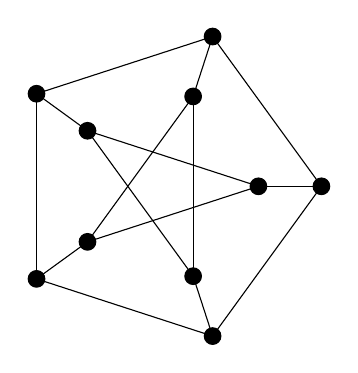
\begin{tikzpicture}
    \pgfmathsetmacro{\pi}{3.14159}
    \foreach \i in {1,...,5}{
      \pgfmathsetmacro{\xia}{1.2*cos(72*\i)}
      \pgfmathsetmacro{\yia}{1.2*sin(72*\i)}
      \pgfmathsetmacro{\xib}{1.2*cos(72*(\i+2))}
      \pgfmathsetmacro{\yib}{1.2*sin(72*(\i+2))}
      \pgfmathsetmacro{\xoa}{2*cos(72*\i)}
      \pgfmathsetmacro{\yoa}{2*sin(72*\i)}
      \pgfmathsetmacro{\xob}{2*cos(72*(\i+1))}
      \pgfmathsetmacro{\yob}{2*sin(72*(\i+1))}
      \draw[fill=black] (\xia,\yia) circle (3pt);
      \draw[fill=black] (\xoa,\yoa) circle (3pt);
      \draw[-] (\xia,\yia) -- (\xib,\yib);
      \draw[-] (\xia,\yia) -- (\xoa,\yoa);
      \draw[-] (\xoa,\yoa) -- (\xob,\yob);}
  \end{tikzpicture}
\end{center}
This graph is completely symmetric in the sense that given any pair of vertices (each representing a line in $\cA$), there is an automorphism of the graph taking one to the other.
In particular, the exceptional divisors are no longer distinguished.

Moreover, given any two pairs of non-adjacent vertices, there is an automorphism of the graph taking one pair to the other.
Each pair of non-adjacent vertices has a unique completion to a collection of four pairwise non-adjacent vertices and thus the lines corresponding to any pair of non-adjacent vertices can be considered as exceptional divisors along with the two additional uniquely determined lines.
In particular, we may blow down the lines corresponding to any pair of non-adjacent vertices to get a surface obtained from $\PP^2$ by blowing up two points.
This procedure gives a toric surface isomorphic to the one given by the fan with rays generated by $(1,0)$, $(0,1)$, $(-1,0)$, $(0,-1)$, and $(-1,-1)$.

Label the five lines of the outer wheel by $L_i$ for $1\le i\le 5$ so that $L_i$ intersects $L_{i-1}$ and $L_{i+1}$ with indices taken modulo 5.
Write $E_i$ for the unique other line intersecting $L_i$.
After blowing down a pair $E_k$ and $E_{k+1}$, we obtain a toric variety as above in which the proper transforms of the lines $L_i$ are precisely the boundary divisors.
It follows that the surface $\cA\setminus(E_k\cup E_{k+1}\cup L_1\cup\cdots\cup L_5)$ is a 2-dimensional toric chart $L_k$ in $\cA$. 
The $L_k$ are precisely the toric charts for a cluster structure on $\cA$.

\bibliographystyle{hyperamsplain}
\bibliography{cluster_symplectic}


\end{document}
